\documentclass[12pt]{ociamthesis}  % default square logo 
%\documentclass[12pt,beltcrest]{ociamthesis} % use old belt crest logo
%\documentclass[12pt,shieldcrest]{ociamthesis} % use older shield crest logo

%load any additional packages

\usepackage{bm}

\usepackage{graphicx}
\graphicspath{ {./images/} }

\usepackage[font=small]{caption}

\usepackage{amssymb}
\usepackage{amsmath}
\usepackage{physics}
\usepackage{titlesec}
\usepackage{lipsum}

\usepackage[bottom]{footmisc}

%\usepackage{newtxtext,newtxmath}

% \usepackage{lmodern}     % set math font to Latin modern math
% \usepackage[T1]{fontenc}
% \renewcommand\rmdefault{ptm}

\usepackage[svgnames]{xcolor}

\usepackage{pgfplots}

\usepackage{tikz}
\usetikzlibrary{arrows.meta}
\usepackage{tikz-3dplot}
\usepackage{tkz-euclide}
\usepackage[ruled,vlined,linesnumbered]{algorithm2e}
\usepackage[margin=25pt]{subcaption}
\usepackage{float}
\usepackage{hyperref}


\newenvironment{changemargin}{%
\begin{list}{}{%
\setlength{\topsep}{0pt}%
\setlength{\topmargin}{1cm}%
\setlength{\listparindent}{\parindent}%
\setlength{\itemindent}{\parindent}%
\setlength{\parsep}{\parskip}%
}%
\item[]}{\end{list}}



\titleformat{\chapter}[block]
  {\normalfont\bfseries}{\LARGE{\thechapter}}{15pt}{\LARGE}[]

  

\titleformat{\section}[block]
{\normalfont\bfseries}{\Large{\thesection}}{15pt}{\Large}[]

%input macros (i.e. write your own macros file called mymacros.tex 
%and uncomment the next line)
%\include{mymacros}

\title{
        Efficient Photorealistic Rendering via Ray-Tracing on GPUs}   %note \\[1ex] is a line break in the title




        
\newcommand{\gapM}
{
        \vspace{5mm}
}

\newcommand{\gapS}
{
        \vspace{2mm}
}

\renewcommand{\u}
{
        \textbf{u}
}
    
\newcommand{\Var}{\mathbb{V}\text{ar}}


%end the preamble and start the document
\begin{document}

%this baselineskip gives sufficient line spacing for an examiner to easily
%markup the thesis with comments
\baselineskip=18pt plus1pt

%set the number of sectioning levels that get number and appear in the contents
\setcounter{secnumdepth}{3}
\setcounter{tocdepth}{3}


\maketitle                  % create a title page from the preamble info
% \begin{dedication}
This thesis is dedicated to\\
 someone\\
for some special reason\\
\end{dedication}        % include a dedication.tex file
% \begin{acknowledgements}
plenty of waffle, plenty of waffle, plenty of waffle, plenty of waffle,
plenty of waffle, plenty of waffle, plenty of waffle, plenty of waffle.
\end{acknowledgements}   % include an acknowledgements.tex file
\begin{abstract}

One of the ultimate goals of the field of computer graphics is to synthesize images that are indistinguishable from photographs. This task, often referred to as photorealistic rendering, is known for being extremely costly, due to the need for a physically-correct simulation of the transport of light in the scene. This project explores methods to accelerate rendering by utilizing the massively parallel computing architectures of GPUs, and creates a renderer whose performance tops some of the best renderers in the academia.

This project focuses on the widely-used rendering algorithm known as path-tracing. The project studies how to maximize the performance of path-tracing on GPUs, and implements state-of-the-art algorithms for the construction and traversal of the data structures used by this algorithm. Besides standard path-tracing, the project also implements a newly emerged variant, where reinforcement learning is used to guide the the selection of light paths. The resulting renderer can robustly handle a variety of real-world materials, complex scene geometry, and difficult lighting situations. Moreover, comprehensive benchmarking indicates that the efficiency of this GPU renderer significantly exceeds other CPU implementations, and is even noticeably faster compared to one of the most academically renowned GPU renderer.

\end{abstract}          % include the abstract


\begin{romanpages}          % start roman page numbering
\tableofcontents            % generate and include a table of contents
%\listoffigures              % generate and include a list of figures
\end{romanpages}            % end roman page numbering

%now include the files of latex for each of the chapters etc
\chapter{Introduction}

\section{Motivation}
May it be glorious space battles with lasers blasting around, or a mountain-high gorilla wrestling a even bigger lizard, modern rendering technologies present our craziest fantasies to our eyes as if they are happening right in front of us. The contemporary film and television industry is highly dependent on this ability of rendering photorealistic images, and alongside the pursuit of wilder stories and imaginations, the scenes to be rendered are becoming increasingly complex and arbitrary.

Despite its importance, the task of photorealistic rendering has a computational cost that is matched by few others. As an example, recent Disney title films could require hundreds of CPU hours just to synthesize a single frame\cite{hyperion}. This immense cost is explained by the fact that there are complex interactions between light rays and scene geometry, and the rendering algorithm must comprehensively and accurately simulate these interactions in order to obtain a realistic image. 

This project studies two orthogonal approaches that both boost the efficiency of rendering. Firstly, this project utilizes GPUs, whose massively parallel architectures allow a large amount of pixels to be processed at the same time. Secondly, from an algorithmic perspective, the project explores how reinforcement learning can be used to guide the algorithm to focus on the ``important'' parts of the scene. The project shows that both methods are indeed effective ways of improving rendering efficiency.

\section{Related Work}

The study of computer graphics began almost as soon as computers with screens are manufactured. In 1980, Whitted\cite{whitted} proposed the algorithm known as \textit{ray-tracing}, which is the algorithmic foundation of almost all photorealistic rendering algorithms used today. However, the version of ray-tracing described by Whitted was not based on a physically plausible model of light, and consequently the images generated was not yet photorealistic. 

The age of photorealism began in 1986 with the visionary work of Kaijiya\cite{rendering_equation}. This paper introduced an integral equation known as \textit{the rendering equation}, which models the power carried by light rays in a physically correct manner. Programs that produce images by computing solutions to this equation are called physically based renderers, and this method have since become the focus of decades of rendering research. In addition, Kaijiya's paper also described a variant of the ray-tracing algorithm known as \textit{path tracing}, which solves the rendering equation using the technique of Monte-Carlo integration. This algorithm is still the core of most of the photorealistic renderers developed and used today, including the renderer implemented in this project.

Path-tracing is a powerful algorithm, but it is too costly\footnote{until perhaps, very recently. See NVIDIA RTX.} to be used for real-time rendering applications such as video games. As a result, real-time applications take a fundamentally different approach to rendering known as rasterization. Modern rasterization-based rendering pipelines can be very-fast: they can render tens or even hundreds of frames per second. However, despite the fact that a range of algorithms\cite{fernando2005percentage}\cite{sloan2002precomputed}\cite{hanrahan1991rapid} exist that aims to make rasterization based algorithms as physically-correct as possible, the images produced by these renderers are still easily recognizable as computer generated. Thus, when the need for image quality dominates that for rendering speed, path-tracing is still the better choice. Notice that however, modern GPUs are designed to optimize for rasterization-based pipelines\footnote{this is beginning to change with NVIDIA RTX} and not for ray-tracing algorithms. 

In a ray tracing algorithm, one of the most costly operations is ray-scene intersection. Intuitively, this is the task of finding the first intersection point between a light ray and the geometries in the scene. A naive linear search across all geometries is of course unacceptably slow, and a range of accelerating data structures have been created. This project employs the data structure of Bounding Volume Hierarchies (BVH), which recursively divides the scene into a tree of axis-aligned bounding boxes. Due to their recursive nature, the construction and traversal of these structures are difficult tasks on GPUs. For this reason, this project studied and implemented a series of GPU BVH techniques published by NVIDIA\cite{bvh_build}\cite{bvh_optimize}\cite{bvh_traversal}.


Ever since the introduction of path-tracing, a variety of algorithms that builds on top of patch-tracing have emerged. The most famous ones include bi-direction path-tracing\cite{veach1997robust}, Metropolis light transport\cite{veach1997robust}\cite{kelemen2002simple}, energy redistribution path-tracing\cite{cline2005energy}, and gradient-domain path-tracing \cite{kettunen2015gradient}. One particularly interesting variant, which uses reinforcement learning to guide the generation of light rays\cite{RLPT}, is studied and implemented in this project. 

One renderer of particular value to the graphics community is the \texttt{pbrt} renderer. Not only is this renderer open-source, it is also accompanied by an entire book\cite{pharr2016physically} which happens to be the most authoritative textbook of physically based rendering. Moreover, because of its popularity, there is a large collection of beautiful scenes defined using \texttt{pbrt}'s input file format. For these reasons, this project decided to support \texttt{pbrt}'s scene definition files, which allows this project to be benchmarked and compared against \texttt{pbrt}.

Most of the ray-tracing renderers used tody, including \texttt{pbrt}, runs on the CPU. However, there is a GPU ray-tracing system known as OptiX\cite{parker2010optix}, which is becoming increasingly popular. Developed by the GPU manufacturer NVIDIA, OptiX is heavily optimized, and provides a friendly ray-tracing library for developers. One famous renderer which uses OptiX as a backbone\footnote{There is also an upcoming 4th version of \texttt{pbrt}, which also supports GPU via OptiX. However, the beta version is still unstable at the time this thesis is written} is the \texttt{Mitsuba} renderer. The GPU rendering routines of this project is implemented from scratch, and its performance will be compared against \texttt{Mitsuba} (and therefore OptiX).

\section{Project Outline}
This project focuses on the GPU parallelization of ray-tracing algorithms for the efficient rendering of photorealistic images. A fully-featured GPU renderer is created, which supports a wide range of geometries, materials, and light sources. At the heart of the renderer are efficient implementations of two algorithms: the original path-tracing algorithm, and a variant of path-tracing guided by reinforcement learning. 

In order to efficiently implement path-tracing, this project implemented state-of-the-art methods of performing ray-scene intersection detection. These includes algorithms for constructing BVH trees in parallel, optimizing the structure of constructed BVHs, and recursion-free methods of tree traversal. The project also makes numerous optimizations that reduces control flow divergences and memory access latencies, so that the resulting implementation maximally utilize the parallel architecture of GPUs.  

This project made the observation that in certain lighting scenarios, the original path-tracing algorithm struggled to converge to a noiseless solution. To alleviate this problem, the project implements a variant of path-tracing, where reinforcement learning is used to guide the selection of light rays. The project investigates how the architecture of the GPU interacts with various aspects of the reinforcement learning routine, and implements a version that allows tens of thousands of GPU threads to efficiently cooperate during learning. 


The renderer created by this project is named \textit{Cavalry}\footnote{The name is inspired by a character in a video game called Overwatch. The character goes by the name ``Tracer'', and refers to herself as the ``Cavalry''.}. It is created mainly using the C++ programing language on the CPU side, and the CUDA language for GPU computing. With a total of over 7 thousand lines, the complete source code of the software can be found at \url{https://github.com/AmesingFlank/Cavalry}, along with some additional information and screenshots.

\chapter{Physically Based Rendering}

In order to generate photorealistic images, renderers must find accurate solutions to the \textit{rendering equation}. This chapter explains the meaning and intuition behind the equation, and describes how it can be solved by the path-tracing algorithm.

\section{The Rendering Equation}

The rendering equation describes the ``strength'' of light at each point in space and in each direction. To formalize the notion of strength, this section begins by introducing a few concepts from the study of radiometry.

\subsection{Radiometry}

In radiometry, there is a hierarchy of quantities that measures the strength of light in different contexts. The first quantity is \textit{radiant flux}, which measures the total energy that travels through a region of space per unit time in the form of electromagnetic radiation. Radiant flux is often denoted by $\Phi$, and its unit of measure is Watts($W$). 

In almost all regions in any scene, the radiant flux is not uniformly distributed, and thus one important quantity is the density of radiant flux with respect to area. This quantity is named \textit{irradiance}, which is denoted by $E$, and measured in power per unit area ($W\cdot m^{-2}$). Intuitively, irradiance measures the amount of light received by a single point in space. For this reason, for a region of space $S$, integrating the irradiance of each point in $S$ gives the total flux through $S$:
\begin{align}
    \Phi(S) = \int_S E(p) dp 
    \label{irradiance integral}
\end{align}

For any point $p$, the irradiance $E(p)$ is not uniform across all directions, and thus it is also important to consider the density of irradiance in each direction $\omega$. This quantity, $L(p,\omega)$, is called \textit{radiance}, and its unit of measure for radiance is power per unit area per unit solid angle ($\text{W}\cdot\text{m}^{-2}\cdot \text{sr}^{-1}$). Radiance is an especially important quantity, because it is a measure of the strength of a single ray of light, identified by its direction $\omega$ and a point $p$ which it passes through. Consequently, radiance is the physical quantity that ray-tracing algorithms constantly operates in. 


In rendering, radiance often appears in the form $L_o(p,\omega)$ or $L_i(p,\omega)$, which mean radiance going out from the point $p$ or entering into it, respectively. More precisely, $L_o(p,\omega)$ represents the radiance that travels from $p$ and outwards in the direction $\omega$, and $L_i(p,\omega)$ represents the incoming radiance that travels towards to $p$ in the direction $-\omega$. The convention $L_i(p,\omega)$ might appear slightly counter-intuitive, since $\omega$ points in the opposite direction as the propagation of energy. However, the convenience of this notation will become apparent when the ray-tracing algorithm is formulated. 



\begin{figure}[H]
\centering
\tikzset{every picture/.style={line width=0.75pt}} %set default line width to 0.75pt        
\begin{tikzpicture}[x=0.75pt,y=0.75pt,yscale=-1,xscale=1]
%uncomment if require: \path (0,300); %set diagram left start at 0, and has height of 300

%Straight Lines [id:da6428603089338014] 
\draw    (70,220) -- (251,220) ;
\draw [shift={(160.5,220)}, rotate = 0] [color={rgb, 255:red, 0; green, 0; blue, 0 }  ][fill={rgb, 255:red, 0; green, 0; blue, 0 }  ][line width=0.75]      (0, 0) circle [x radius= 3.35, y radius= 3.35]   ;
%Straight Lines [id:da0998330538982608] 
\draw    (160.5,220) -- (218.58,162.41) ;
\draw [shift={(220,161)}, rotate = 495.24] [color={rgb, 255:red, 0; green, 0; blue, 0 }  ][line width=0.75]    (10.93,-3.29) .. controls (6.95,-1.4) and (3.31,-0.3) .. (0,0) .. controls (3.31,0.3) and (6.95,1.4) .. (10.93,3.29)   ;
%Straight Lines [id:da7334390340946089] 
\draw    (325,221) -- (506,221) ;
\draw [shift={(415.5,221)}, rotate = 0] [color={rgb, 255:red, 0; green, 0; blue, 0 }  ][fill={rgb, 255:red, 0; green, 0; blue, 0 }  ][line width=0.75]      (0, 0) circle [x radius= 3.35, y radius= 3.35]   ;
%Straight Lines [id:da024849495612862427] 
\draw    (480,160) -- (416.95,219.63) ;
\draw [shift={(415.5,221)}, rotate = 316.6] [color={rgb, 255:red, 0; green, 0; blue, 0 }  ][line width=0.75]    (10.93,-3.29) .. controls (6.95,-1.4) and (3.31,-0.3) .. (0,0) .. controls (3.31,0.3) and (6.95,1.4) .. (10.93,3.29)   ;
%Image [id:dp8436986937138125] 
\draw (161,245) node  {
\includegraphics[width=27pt,height=30pt]{lightbulb.png}};
%Image [id:dp5859653893638117] 
\draw (498,154) node  {
\includegraphics[width=27pt,height=30pt]{lightbulb.png}};

% Text Node
\draw (181,232) node [anchor=north west][inner sep=0.75pt]   [align=left] {$\displaystyle p$};
% Text Node
\draw (224,143) node [anchor=north west][inner sep=0.75pt]   [align=left] {$\displaystyle q$};
% Text Node
\draw (436,233) node [anchor=north west][inner sep=0.75pt]   [align=left] {$\displaystyle p$};
% Text Node
\draw (519,141) node [anchor=north west][inner sep=0.75pt]   [align=left] {$\displaystyle q$};


\end{tikzpicture}

\caption{Example: consider two points $p$, $q$, and $\omega=\frac{q-p}{|q-p|}$. On the left, the radiance sent from $p$ to $q$ is $L_o(p,\omega)$. On the right, the radiance received by $p$ from $q$ is $L_i(p,\omega)$.}
\end{figure}
Similar to equation \ref{irradiance integral}, which expresses flux as an integral of irradiance, it's also possible to obtain the incoming irradiance $E(p)$ by an integral across the incoming radiance from each direction. More precisely, the following relationship holds:
\begin{align}
    E(p) = \int_\Omega L_i(p,\omega_i)\cos\theta_id\omega_i
    \label{radiance integral}
\end{align}
Here, the support $\Omega$ is often a sphere or hemisphere of possible incoming direction, and the angle $\theta_i$ represents the angle between $\omega_i$ and the surface normal. The cosine term accounts for the fact that for incoming rays that are not perfectly perpendicular to the surface, the differential area illuminated by the ray is multiplied by a factor $\frac{1}{\cos\theta_i}$, and thus the contribution per unit area should be multiplied by $\cos\theta_i$. 
\begin{figure}[H]
    \centering
  



    \tikzset{every picture/.style={line width=0.75pt}} %set default line width to 0.75pt        

    \begin{tikzpicture}[x=0.75pt,y=0.75pt,yscale=-1,xscale=1]
    %uncomment if require: \path (0,300); %set diagram left start at 0, and has height of 300
    
    %Straight Lines [id:da170514078900192] 
    \draw    (54,230) -- (176,230) ;
    \draw [shift={(115,230)}, rotate = 0] [color={rgb, 255:red, 0; green, 0; blue, 0 }  ][fill={rgb, 255:red, 0; green, 0; blue, 0 }  ][line width=0.75]      (0, 0) circle [x radius= 3.35, y radius= 3.35]   ;
    %Straight Lines [id:da016015541896946983] 
    \draw    (100,160) -- (130,160) ;
    %Straight Lines [id:da2875279917672757] 
    \draw  [dash pattern={on 0.84pt off 2.51pt}]  (100,160) -- (100,230) ;
    %Straight Lines [id:da4948721440011248] 
    \draw  [dash pattern={on 0.84pt off 2.51pt}]  (130,160) -- (130,230) ;
    %Straight Lines [id:da6791345652096885] 
    \draw [line width=2.25]    (100,230) -- (130,230) ;
    %Straight Lines [id:da17937256958328818] 
    \draw    (249,230) -- (371,230) ;
    \draw [shift={(310,230)}, rotate = 0] [color={rgb, 255:red, 0; green, 0; blue, 0 }  ][fill={rgb, 255:red, 0; green, 0; blue, 0 }  ][line width=0.75]      (0, 0) circle [x radius= 3.35, y radius= 3.35]   ;
    %Straight Lines [id:da5726229973180355] 
    \draw    (358.31,159.71) -- (379.42,181.02) ;
    %Straight Lines [id:da01972159484297009] 
    \draw  [dash pattern={on 0.84pt off 2.51pt}]  (358.31,159.71) -- (286,230) ;
    %Straight Lines [id:da8044979993297667] 
    \draw  [dash pattern={on 0.84pt off 2.51pt}]  (379.42,181.02) -- (329.69,230.29) ;
    %Straight Lines [id:da7389754977606782] 
    \draw [line width=2.25]    (286,230) -- (332,230) ;
    %Straight Lines [id:da7593939440598445] 
    \draw    (310,230) -- (310,161) ;
    \draw [shift={(310,159)}, rotate = 450] [color={rgb, 255:red, 0; green, 0; blue, 0 }  ][line width=0.75]    (10.93,-3.29) .. controls (6.95,-1.4) and (3.31,-0.3) .. (0,0) .. controls (3.31,0.3) and (6.95,1.4) .. (10.93,3.29)   ;
    %Straight Lines [id:da5048921054355329] 
    \draw    (310,230) -- (359.59,180.41) ;
    \draw [shift={(361,179)}, rotate = 495] [color={rgb, 255:red, 0; green, 0; blue, 0 }  ][line width=0.75]    (10.93,-3.29) .. controls (6.95,-1.4) and (3.31,-0.3) .. (0,0) .. controls (3.31,0.3) and (6.95,1.4) .. (10.93,3.29)   ;
    %Curve Lines [id:da665946044320908] 
    \draw    (310,215) .. controls (315,212) and (319,213) .. (321,218) ;
    
    % Text Node
    \draw (107,140) node [anchor=north west][inner sep=0.75pt]   [align=left] {$\displaystyle A$};
    % Text Node
    \draw (102,239) node [anchor=north west][inner sep=0.75pt]   [align=left] {$\displaystyle A_{1}$};
    % Text Node
    \draw (373,154) node [anchor=north west][inner sep=0.75pt]   [align=left] {$\displaystyle A$};
    % Text Node
    \draw (297,239) node [anchor=north west][inner sep=0.75pt]   [align=left] {$\displaystyle A_{2}$};
    % Text Node
    \draw (315,197) node [anchor=north west][inner sep=0.75pt]  [font=\small] [align=left] {$\displaystyle \theta $};
    
    
    \end{tikzpicture}
    

\caption{Example: on the right, the differential area $A_2$ illuminated by the ray is larger, because the ray is not perpendicular to the plane.}    
\end{figure}


\subsection{The BRDF}

In order to model the outgoing radiances at each point, it is essential to account for the fact that surfaces reflect incoming light: for any direction $\omega_i$, the incoming radiance $L_i(p,\omega_i)$ contributes to the outgoing radiance $L_o(p,\omega_o)$ of another direction $\omega_o$. This relationship is captured by the bi-directional reflectance distribution function (BRDF), written as $f_r(p,\omega_o,\omega_i)$. Formally, the BRDF is defined as 
\begin{align}
    f_r(p,\omega_o,\omega_i) = \frac{dL_o(p,\omega_o)}{dE(p,\omega_i)}
    \label{BRDF def 1}
\end{align}
where $dE(p,\omega_i)$ represents the differential incoming irradiance at the direction $\omega_i$.

Using equation \ref{radiance integral}, it can be derived that 
\begin{align}
    dE(p,\omega_i) = L_i(p,\omega_i)\cos\theta_id\omega_i
\end{align}
which allows equation \ref{BRDF def 1} to be re-written as
\begin{align}
    f_r(p,\omega_o,\omega_i) = \frac{dL_o(p,\omega_o)}{L_i(p,\omega_i)\cos\theta_id\omega_i}
\end{align}
From this, it's straightforward to show that, for some $C$,
\begin{align}
    L_o(p,\omega_o) = \int_\Omega L_i(p,\omega_i)f_r(p,\omega_o,\omega_i)\cos\theta_id\omega_i + C
    \label{reflection plus C}
\end{align}

The BRDF of a surface completely decides how it reflects light, which is a crucial factor of its appearances. Different materials in the real world have drastically different BRDFs, and it's vital for a physically based renderer to accurately implement these functions. A family of BRDFs known for their physical accuracy are the Microfacet BRDFs\cite{cook1982reflectance}, which are well implemented by this project. Unfortunately, due to their complexity, details of these BRDFs could not be described here. 


In order to fully model $L_o(p,\omega_o)$, it remains to describe the term $C$ in equation \ref{reflection plus C}. Surfaces in the real world sends outgoing radiances for two reasons only: they might emit light actively, and they reflect incoming light. Equation \ref{reflection plus C} already includes the reflected radiances, and thus it only remains to include actively emitted light. Writing $L_e(p,\omega_o)$ for the actively emitted radiance from $p$ towards the direction $\omega_o$, the following equation completely describes $L_o$:
\begin{align}
    L_o(p,\omega_o) = L_e(p,\omega_o) + \int_\Omega L_i(p,\omega_i)f_r(p,\omega_o,\omega_i)\cos\theta_id\omega_i
    \label{rendering equation}
\end{align}
which is the famous rendering equation, originally proposed by Kaijiya\cite{rendering_equation}. 


Under the assumption that radiance is constant along each ray, the incoming radiance $L_i(p,\omega_i)$ can be equated with the outgoing radiance from another point, $q$, as illustrated below.
\begin{figure}[H]
    \centering
    


\tikzset{every picture/.style={line width=0.75pt}} %set default line width to 0.75pt        

\begin{tikzpicture}[x=0.75pt,y=0.75pt,yscale=-1,xscale=1]
%uncomment if require: \path (0,300); %set diagram left start at 0, and has height of 300

%Straight Lines [id:da05220876887007719] 
\draw    (30,260) -- (211,260) ;
\draw [shift={(120.5,260)}, rotate = 0] [color={rgb, 255:red, 0; green, 0; blue, 0 }  ][fill={rgb, 255:red, 0; green, 0; blue, 0 }  ][line width=0.75]      (0, 0) circle [x radius= 3.35, y radius= 3.35]   ;
%Straight Lines [id:da8868681333199677] 
\draw    (150,230.5) -- (121.91,258.59) ;
\draw [shift={(120.5,260)}, rotate = 315] [color={rgb, 255:red, 0; green, 0; blue, 0 }  ][line width=0.75]    (10.93,-3.29) .. controls (6.95,-1.4) and (3.31,-0.3) .. (0,0) .. controls (3.31,0.3) and (6.95,1.4) .. (10.93,3.29)   ;
%Image [id:dp7926495246340768] 
\draw (232,169) node  {
\includegraphics[width=27pt,height=30pt]{lightbulb.png}};
%Straight Lines [id:da34057240843922076] 
\draw  [dash pattern={on 0.84pt off 2.51pt}]  (150,230.5) -- (180,200) ;
%Straight Lines [id:da8846910740201797] 
\draw    (210,170) -- (181.41,198.59) ;
\draw [shift={(180,200)}, rotate = 315] [color={rgb, 255:red, 0; green, 0; blue, 0 }  ][line width=0.75]    (10.93,-3.29) .. controls (6.95,-1.4) and (3.31,-0.3) .. (0,0) .. controls (3.31,0.3) and (6.95,1.4) .. (10.93,3.29)   ;

% Text Node
\draw (141,272) node [anchor=north west][inner sep=0.75pt]   [align=left] {$\displaystyle p$};
% Text Node
\draw (255,155) node [anchor=north west][inner sep=0.75pt]   [align=left] {$\displaystyle q$};
% Text Node
\draw (123,163) node [anchor=north west][inner sep=0.75pt]   [align=left] {$\displaystyle L_{o}( q,-\omega _{i})$};
% Text Node
\draw (64,224) node [anchor=north west][inner sep=0.75pt]   [align=left] {$\displaystyle L_{i}( p,\omega _{i})$};


\end{tikzpicture}

\end{figure} 
Thus, defining the ray-tracing function $t(p,\omega_i)$ that computes the first surface point $q$ intersected by a ray originated from $p$ and travels in the direction $\omega_i$, the rendering equation is re-written as:
\begin{align}
    L_o(p,\omega_o) = L_e(p,\omega_o) + \int_\Omega L_o(t(p,\omega_i),-\omega_i)f_r(p,\omega_o,\omega_i)\cos\theta_id\omega_i
    \label{rendering equation with cast}
\end{align}

Finding solutions to this equation is the ultimate goal of rendering, because the job of any renderer is to compute the amount of radiance received by a hypothetical camera placed in the scene. For each point $p$ visible from the camera, the rendering algorithm must compute $L_o(p,\omega_o)$, where $\omega_o$ points from $p$ towards the camera. 

\section{Monte Carlo Integration}

Equation \ref{rendering equation with cast} cannot be solved analytically for all but the simplest scenes. Thus, rendering software solve the equation numerically using the method of Monte Carlo integration. Given an integral
\begin{align*}
    I = \int_\Omega f(x) dx,
\end{align*}
the Monte Carlo estimator randomly samples $N$ points $x_1,...,x_n\in \Omega$ according to some distribution $D$, and computes
\begin{align}
    I_N = \frac{1}{N}\sum_{i=1}^{N} \frac{f(x_i)}{p(x_i)}
    \label{monte carlo estimator}
\end{align}
where $p(x_i)$ is the probability density of sampling $x_i$ according to $D$. It can be proved that this indicator is both unbiased $(E[I_N]=I)$ and consistent $(\lim_{N\to\infty}I_N = I)$. When applied to the rendering equation, the support $\Omega$ is the sphere or hemisphere of directions, and the function $f$ is computed by recursively estimating $L_o$, and then multiplying by the BRDF and the cosine of the direction.

\subsection{Importance Sampling}

In rendering, the variance $\Var[I_N]$ of the Monte Carlo estimator manifest in the form of random noise in the resulting image. Thus, variance reduction techniques are vital for rendering high-quantity images efficiently. One of the most important such techniques is importance sampling.

In the monte carlo estimator, the distribution $D$ used can be an arbitrary distribution. However, different distributions can lead to dramatically different variances. Importance sampling uses the fact that, informally, the variance $\Var[I_N]$ is reduced as the shape of the PDF $p(x)$ becomes similar to the shape of the integrand $f(x)$. As an example, consider when the PDF is 
$$ 
p(x)=\frac{f(x)}{\int_\Omega f(x') dx'}.
$$ 
In this case, $p$ is always proportional to $f$, and the variance of the estimator is
\begin{align*}
\Var[I_N]
&= \frac{1}{N}\Var_{x\sim D}\left[\frac{f(x)}{p(x)}\right]\\
&= \frac{1}{N}\Var_{x\sim D}\left[\int_\Omega f(x') dx'\right]\\
&=0
\end{align*}
It is of course infeasible to obtain a perfectly proportional PDF, because doing so requires computing the value of $\int_\Omega f(x') dx'$, which is the value to be estimated in the first place. However, even if $p$ is similar in shape to $f$, variance can still be reduced.

\subsection{Multiple Importance Sampling}
\label{subsection MIS}
When solving the rendering equation, the integrand is the product of two factors: the incoming radiance $L_o(t(p,\omega_i),-\omega_i)$, and the reflectance $f_r(p,\omega_o,\omega_i)\cos\theta_i$. More generally, the renderer is solving an integration of the form
$$
I = \int_\Omega f(x)g(x)dx
$$

In this case, if the renderer were to perform importance sampling to estimate this integral according to distributions based on either $f$ or $g$, one of these two will often perform poorly\cite{pharr2016physically}. This is exactly the issue addressed by the technique of multiple importance sampling, or MIS.

The basic idea of MIS is that, when estimating an integral, samples should be drawn from multiple distributions, chosen in the hope that at least one will match the shape of the integrand well. MIS provides a method of weighting the samples from each distribution that eliminates large variance spikes due to mismatches between the integrand and the sampling density. More precisely, given a PDF $p_f$ that is a good match for $f$, and $p_g$ that is a good match for $g$, MIS proposes to $N$ samples $x_1,...,x_N$ from $p_f$, and $y_1,...,y_N$ from $p_g$, and apply the alternative Monte Carlo estimator:
\begin{align}
    I_N = \frac{1}{N} \sum_{i=1}^{N} \frac{f(x_i)g(x_i)w_f(x_i)}{p_f(x_i)} + \frac{f(y_i)g(y_i)w_g(y_i)}{p_g(y_i)}
    \label{MIS}
\end{align}
where the weights $w_f$ and $w_g$ are defined by
\begin{align*}
    w_s(x) = \frac{p_f(x)^2}{p_f(x)^2+p_g(x)^2}
\end{align*}
A full recount of why this weighting scheme reduces variance can be found in \cite{pharr2016physically}. 

To apply MIS when solving the rendering equation, the renderer samples from a PDF $p_{rad}$ that matches to the incoming radiance $L_o(t(p,\omega_i),-\omega_i)$, and another PDF $p_{ref}$ that matches the reflection term $f_r(p,\omega_o,\omega_i)\cos\theta_i$. In the implementation of this project, $p_{rad}$ is a distribution which only samples $\omega_i$ that points to a light source, which is often much brighter than surfaces that indirectly reflects light. For $p_{ref}$, the project implemented specific sampling routings for each individual BRDF, thereby maximizing the similarity between the PDF and the BRDF of each sample point.


\section{The Path Space Formulation}
The rendering equation as written in equation \ref{rendering equation with cast} is inconvenient for deriving algorithms, because the relationship between geometries in the scene is implicit in the ray-tracing function $t(p,\omega_i)$. This section rewrites the equation into a from that makes this relationship more explicit.

Firstly, equation \ref{rendering equation with cast} is to be transformed from an integral over directions into an integral over area. Specifically, the variable of integration $\omega_i$, which represents an incoming direction, is to be replaced by a point $p_{src}$, which represents the source of the incoming ray. To achieve this, for any pair of mutually visible points $p,p'$, define 
\begin{align*}
    L_o(p'\to p) = L_o(p',\omega)\\
    L_e(p'\to p) = L_e(p',\omega)
\end{align*}
where $\omega = \frac{p-p'}{|p-p'|}$. Similarly, for three points $p,p',p''$, such that $p$ is visible from $p'$ and $p'$ is visible from $p''$, the BRDF at $p'$ is written as
\begin{align*}
    f_r(p''\to p'\to p) = f_r(p',\omega_o,\omega_i)
\end{align*} 
where $\omega_i = \frac{p''-p'}{|p''-p'|}$ and $\omega_o = \frac{p-p'}{|p-p'|}$.

Note that, since not all points $p_{src}$ is visible from $p$, the integrand needs to include a visibility term $V(p,p_{src})$, which takes the value 1 if $p_{src}$ is visible from $p$, and 0 otherwise. Furthermore, the change of variable also incurs a Jacobian term, which is $\frac{\cos\theta'}{|p-p_{src}|^2}$, with $\theta'$ being the angle between the incoming ray and the surface normal at $p_{src}$. Use these terms, equation \ref{rendering equation with cast} is rewritten so that for a ray from a point $p$ to the destination $p_{dest}$, the radiance is computed by
\begin{align*}
    L_o(p\to p_{dest}) =~ &L_e(p\to p_{dest}) \\
    &+ \int_A f_r(p_{src}\to p\to p_{dest}) L_o(p_{src}\to p)  V(p,p_{src}) \frac{cos\theta\cos\theta'}{|p-p_{src}|^2} d p_{src}
\end{align*} 
where $A$ is the domain of all surface points in the scene. To simplify notation, write the term $G(p,p_{src})$ as $V(p,p_{src}) \frac{cos\theta\cos\theta'}{|p-p_{src}|^2}$, the equation becomes
\begin{align*}
    L_o(p\to p_{dest}) =~ &L_e(p\to p_{dest}) \\
    &+ \int_A f_r(p_{src}\to p\to p_{dest}) L_o(p_{src}\to p)  G(p,p_{src})  d p_{src}
\end{align*} 

The equation above is referred to as the surface form light transport equation, and it can be interpreted as a recursive definition for $L_o$. Naturally, one can expand this recursive definition, and obtain an infinite sum:
\begin{align*}
    L_o(p_1\to p_0) =
    &L_e(p_1\to p_0)\\
    &+ \int_A L_e(p_2\to p_1)f_r(p_2\to p_1\to p_0)G(p_2,p_1) dp_2\\
    &+ \int_A \int_A L_e(p_3\to p_2)f_r(p_3\to p_2\to p_1) G(p_3,p_2)f(p_2\to p_1\to p_0)G(p_2,p_1) ~ dp_3dp_2\\
    &+~...
\end{align*}
Here, each term represents the radiance contributed by paths of increasing length. For a path with $n$ reflection points, the source emission is $L_e(p_{n+1}\to p_{n})$, and it is weighted by a throughput term $T_n$, which is the product of the $f_r$ and $G$ at each reflection point:
\begin{align*}
    T_n = \prod_{i=1}^{n} f_r(p_{n+1}\to p_n\to p_{n-1})G(p_{n+1},p_n)
\end{align*}
Substituting this into the previous equation gives
\begin{align*}
    L_o(p_1\to p_0) = \sum_{n=0}^{\infty} \underbrace{\int_A \int_A...\int_A}_{n} L_e(p_{n+1}\to p_{n})T_n dp_{n}dp_{n-1}...dp_1
\end{align*}


Notice that, the throughput term $T_n$ computes the portion of radiance that remains after $n$ reflections, which tends to decrease exponentially as $n$ increases. For this reason, it is natural to only consider the first few terms of this infinite sum (see figure \ref{fig maxdepth}). More precisely, given a maximum amount of reflections $MaxDepth$, the radiance $L_o(p_1\to p_0)$ can be estimated by 
\begin{align}
    L_o(p_1\to p_0) = \sum_{n=0}^{MaxDepth} \underbrace{\int_A \int_A...\int_A}_{n} L_e(p_{n+1}\to p_{n})T_n dp_{n}dp_{n-1}...dp_1
    \label{rendering equation path tracing}
\end{align}

If a Monte Carlo estimator is used to approximate the integrals, the above formula becomes a recipe for a practical algorithm for computing radiances. This leads to the famous algorithm known as path-tracing, which is described in the next section.

\begin{figure}[H]
    \centering
    
    \begin{minipage}[t]{.45\textwidth}
        \centering
        \vspace{0pt}
        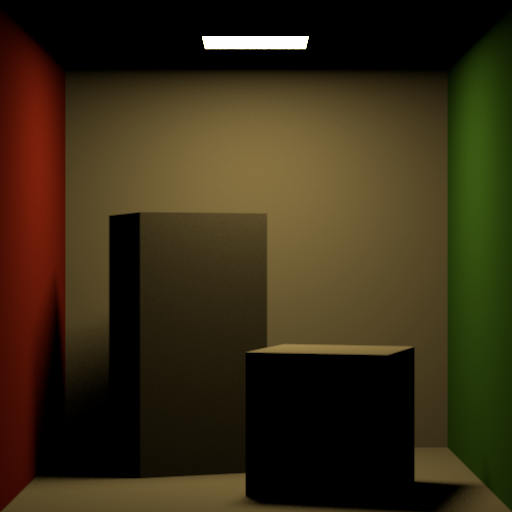
\includegraphics[width=.96\textwidth]{cornell_d1.png}
        \subcaption{$MaxDepth=1$}
    \end{minipage}
    \begin{minipage}[t]{.45\textwidth}
        \centering
        \vspace{0pt}
        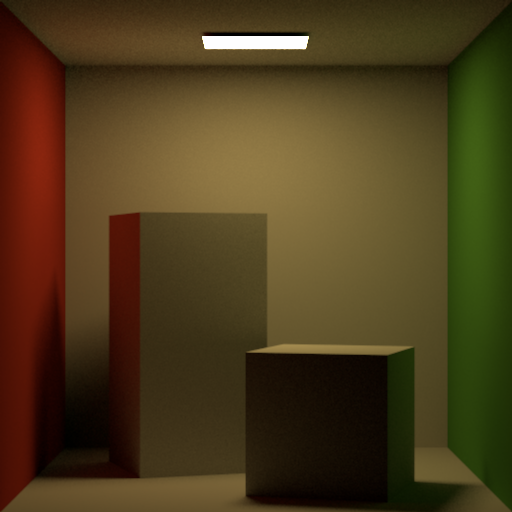
\includegraphics[width=.96\textwidth]{cornell_d2.png}
        \subcaption{$MaxDepth=2$}
    \end{minipage}

    \vspace{0.3cm}

    \begin{minipage}[t]{.45\textwidth}
        \centering
        \vspace{0pt}
        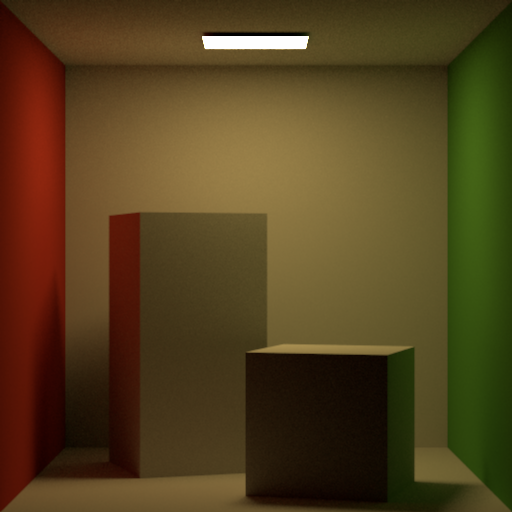
\includegraphics[width=.96\textwidth]{cornell_d3.png}
        \subcaption{$MaxDepth=3$}
    \end{minipage}
    \begin{minipage}[t]{.45\textwidth}
        \centering
        \vspace{0pt}
        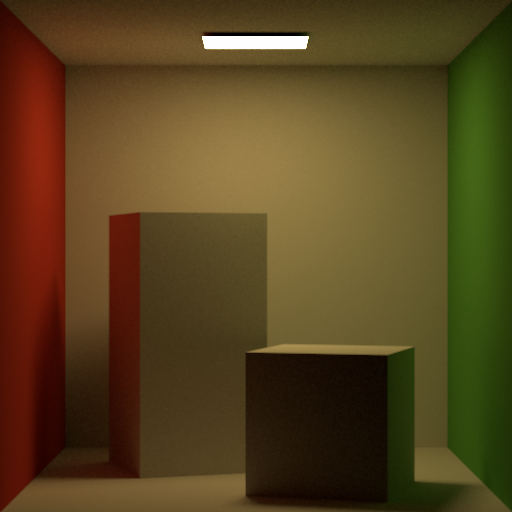
\includegraphics[width=.96\textwidth]{cornell_d4.png}
        \subcaption{$MaxDepth=4$}
    \end{minipage}
    \caption{Effect of increasing $MaxDepth$}
    \label{fig maxdepth}
\end{figure}

\section{The Path-Tracing Algorithm}

The path-tracing algorithm is parameterized by an integer, $spp$, which stands for samples per pixel. The algorithm samples $spp$ random points on each pixel to be rendered, and generate an initial ray corresponding to each sample point. Starting from the ray, the algorithm constructs $MaxDepth*2$ paths of increasing length, and accumulates the radiances carried by these paths. These radiances are combined by a MIS Monte Carlo estimator, which decides the final value of the pixel.

The path tracing algorithm generates paths incrementally, starting from the camera location $p_0$. At each surface point $p_n$, the algorithm samples an incoming direction (for $p_{1}\to p_0$, the direction is fixed by the configuration of the camera), and traces the incoming ray to find $p_{n+1}$. If the point $p_{n+1}$ emits light actively, then this constitutes a path of $n$ reflection point. Moreover, $p_{n+1}$ also serves as the next reflection point, so the algorithm samples a point $p_{light}$ that illuminates $p_{n+1}$, and the radiance can be passed back to $p_0$ through a chain of reflections.


More precisely, the path tracing algorithm works as follows:


\begin{algorithm}[H]
    \label{Path Tracing}
    \SetKwProg{Fn}{Function}{:}{end}
    \ForEach{\upshape pixel in the image}{
        \For{\upshape $i$ from 1 to $spp$}{
            Generate the initial ray $r_0$ going out of the camera position $p_0$\;
            \For{\upshape $n$ from 1 to $MaxDepth$}{
                Find $p_n$ by computing the intersection between $r_{n-1}$ and the scene\;

                \If{\upshape $p_n$ is on a light source}{
                    Accumulate the radiance of the path $p_n\to p_{n-1}\to ... \to p_0$\;
                }
                
                Sample a point $p_{light}$ on a light source\;

                
                \If{\upshape the ray $p_{light}\to p_n$ is not occluded}{
                    Accumulate the radiance of the path $p_{light}\to p_n\to ... \to p_0$\;
                }
                
                Sample a direction $\omega_i$ from a PDF matching the BRDF at $p_n$\;

                Generate the ray $r_{n}$, originated at $p_n$ and points towards $\omega_i$\;
                
            }
            
        }
        Combine radiances computed by all samples to obtain final color of pixel\;
    }
    \caption{Path Tracing}
\end{algorithm}

~

Notice that, line 7 and 10 are two different ways a light emitter can illuminate $p_{n-1}$, and these two paths exactly correspond to the MIS procedure described in section \ref{subsection MIS}. When accumulating their radiances, the MIS weight should be applied.


For each pixel, the algorithm estimates its color using a total of $spp*2*MaxDepth$ paths. Thus, as the parameter $spp$ increases, the variance of the Monte Carlo Estimator is reduced, which implies less noise in the rendered image. The following figure illustrates this effect.


\begin{figure}[H]
    \centering
    
    \begin{minipage}[t]{.45\textwidth}
        \centering
        \vspace{0pt}
        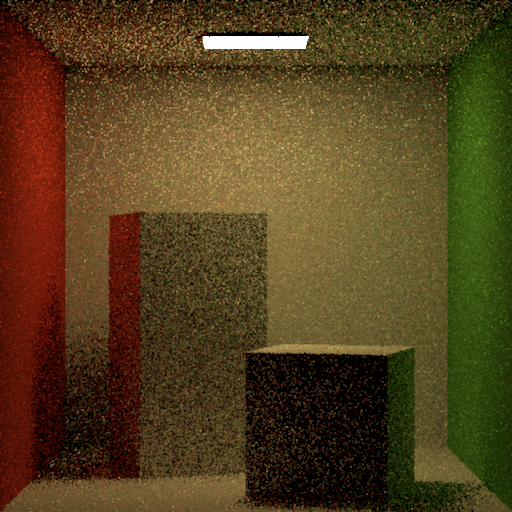
\includegraphics[width=.96\textwidth]{cornell_spp1.png}
        \subcaption{$spp=1$}
    \end{minipage}
    \begin{minipage}[t]{.45\textwidth}
        \centering
        \vspace{0pt}
        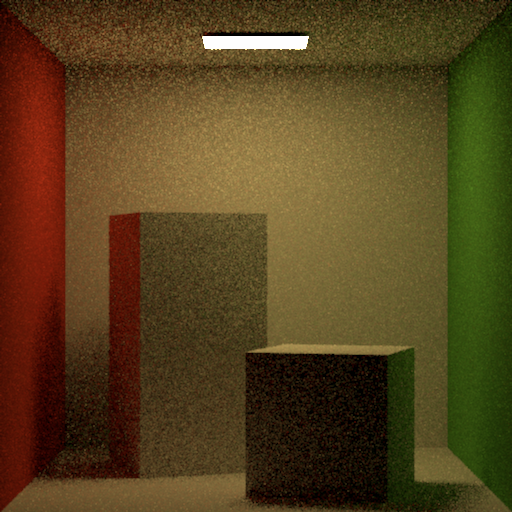
\includegraphics[width=.96\textwidth]{cornell_spp4.png}
        \subcaption{$spp=4$}
    \end{minipage}

    \vspace{0.3cm}

    \begin{minipage}[t]{.45\textwidth}
        \centering
        \vspace{0pt}
        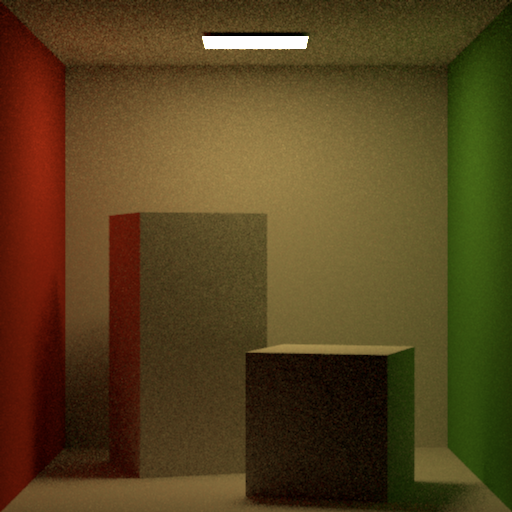
\includegraphics[width=.96\textwidth]{cornell_spp16.png}
        \subcaption{$spp=16$}
    \end{minipage}
    \begin{minipage}[t]{.45\textwidth}
        \centering
        \vspace{0pt}
        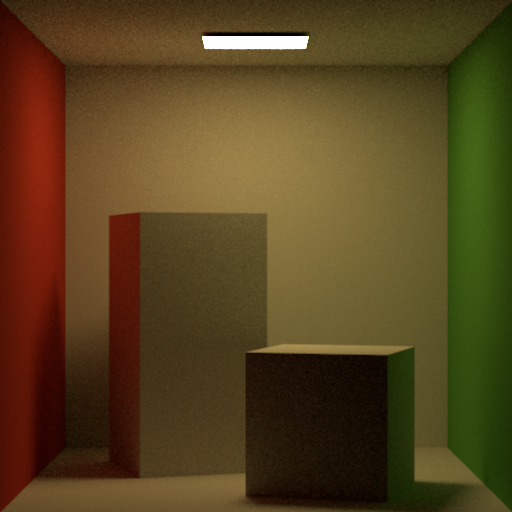
\includegraphics[width=.96\textwidth]{cornell_spp64.png}
        \subcaption{$spp=64$}
    \end{minipage}
    \caption{Effect of increasing $MaxDepth$}
    \label{fig maxdepth}
\end{figure}

For a typical scene, $spp$ is required to be at least 1024 in order to reduce noise down to an inconceivable level. Common images to be rendered consists of around 1 million pixels, thus around 1 billion pixel samples are often needed. Moreover, each ray generated in the algorithm needs to tested for intersection with the entire scene, which often consists of millions of geometric primitives. The next chapter of this report will discuss how this project copes with this humongous amount of computation and implements an efficient path-tracing renderer.


\chapter{Implementing Path-Tracing}
\label{chapter implementation}

To maximize rendering efficiency, this projects implements path-tracing with parallelization on GPUs. This chapter begins with an introduction to GPU computing, and then discusses some of the most impactful performance optimizations employed by this project. These include careful structuring of GPU kernels, avoidance of performance degradation caused by polymorphism, and most importantly, usage of Bounding Volume Hierarchies to accelerate intersection detections.

\section{The CUDA Programming Model}

Originally built for real-time rendering, GPUs can handle a massive amount of geometries and pixels in parallel. The ability to do massively parallel computation motivated GPGPU (General-Purpose GPU) programming models, which became significantly useful for high performance computing. The software in this project is written using the CUDA programming model, developed by the NVIDIA Corporation.

CUDA employs the execution model known as SIMT (Single Instruction Multiple Threads). In this model, a large amount of threads are spawned simultaneously, each running the same code on different data. CUDA threads are organized in groups of 32, known as \textit{warps}. Each thread must execute the same instructions as the others in the same warp, or remain idle. When the threads within a warp access the memory, the entire warp can be paused and swapped out, so that a different warp can execute before the memory access finishes. Using this mechanism, the GPU hides memory access latencies by allowing very fast context switching. As a result, each physical core in the GPU can simultaneously handle multiple logical threads.

As an example, the GPU used for development of this project is an NVIDIA GTX1060 Mobile, which contains 10 \textit{Streaming Multiprocessors}, each of which consists of 128 CUDA cores. Each streaming multiprocessors can have up to 2048 resident threads, giving a total of 20480 threads that can be simultaneously handled. Even though each GPU thread is not as fast as a CPU thread, the aggregated performance of the CUDA cores can still be many times faster than the CPU.

% \begin{figure}[H]
%     \centering
%     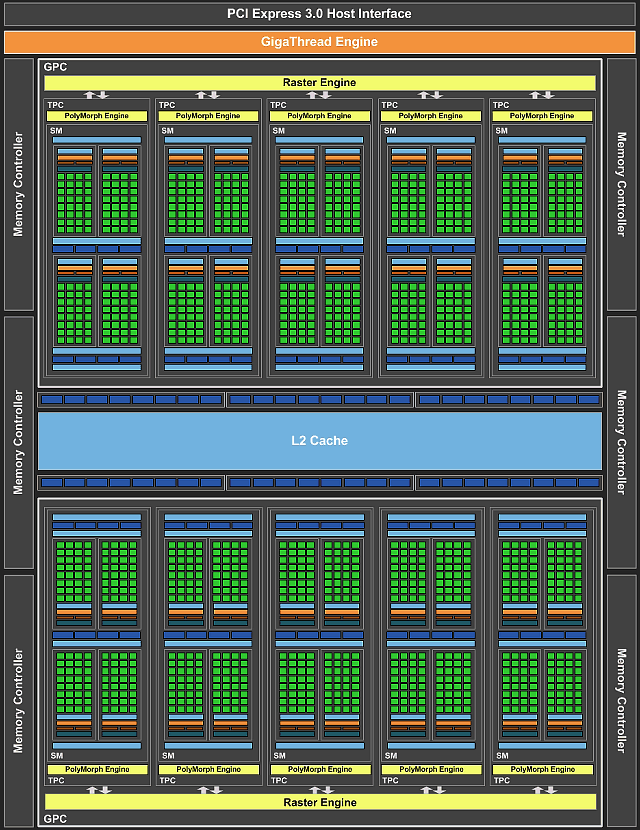
\includegraphics[width=11cm]{gp106}
%     \caption{Architecture of a GTX 1060 (GP106), showing its 10 streaming multiprocessors, each containing 128 CUDA cores. Image credit \cite{pascal}}
%     \label{figure GTX1060}
% \end{figure}
%https://images.nvidia.com/content/pdf/tesla/whitepaper/pascal-architecture-whitepaper.pdf



\section{Wavefront Path-Tracing}
In CUDA, a parallel GPU function that is invoked by the CPU is called a GPU \textit{kernel}. When implementing algorithm \ref{Path Tracing} on GPUs, the most straightforward method is to implement the loop body (lines 3 to 12) as a GPU kernel, and invoke it for all pixel samples in parallel. This pattern of programming, where the entire computation is embodied in a single GPU kernel, is called the \textit{Megakernel}\cite{megakernel} approach.

In contrast to megakernels, the \textit{Wavefront} programming divides the computation into many small kernels, where intermediate results are explicitly stored in memory. The CPU invokes these kernels one after another. On GPUs, regions of code that uses a large amount of registers or has a high control flow divergence can significantly hurt the parallelization of the entire kernel, and thus the wavefront pattern can effectively contain these regions of code into separate kernels, so that the performance of the other kernels remain unaffected. However, the wavefront pattern incurs additional overhead by requiring more CPU-GPU communication, and memory IOs.

The project carried out numerous experiments to find an optimal way of dividing the rendering work into wavefronts. In the end, the program implemented is structured as indicated by the following pseudo-code:

\begin{algorithm}[H]
    \label{algo wavefront Path Tracing}
    \SetKwProg{Fn}{Function}{:}{end}
    \ForEach{\upshape pixel sample \textbf{in a parallel kernel}}{
        generate the initial ray $r_0$ going out of the camera position $p_0$\;
    }
    \For{\upshape $n$ from 1 to $MaxDepth$}{
        \ForEach{\upshape previously generated ray $r$ \textbf{in a parallel kernel}}{
            Find $p_n$ by computing the intersection between $r$ and the scene\;
            \If{\upshape $p_n$ is on a light source}{
                Accumulate the radiance of the path $p_n\to p_{n-1}\to ... \to p_0$\;
            }
        }
        \ForEach{\upshape newly found $p_n$ \textbf{in a parallel kernel}}{
            Sample a point $p_{light}$ on a light source\;
            Test whether the ray $p_{light}\to p_n$ occluded by some geometry\;
        }
        \ForEach{\upshape unoccluded $p_{light}\to p_{n}$ \textbf{in a parallel kernel}}{
            Accumulate the radiance of the path $p_{light}\to p_n\to ... \to p_0$\;
        }
        \ForEach{\upshape $p_n$ \textbf{in a parallel kernel}}{
            Sample a direction $\omega_i$ from a distribution matching the BRDF at $p_n$\;
            Generate a new ray, originated at $p_n$ and travels in the direction of $\omega_i$\;
        }
    }
    \caption{Wavefront Path Tracing}
\end{algorithm}

~

It was found that compared to a naive Megakernel implementation, this wavefront implementation is almost twice as fast.

\section{Polymorphism}
In GPU programming, a common source of performance degradation is dynamic-dispatch polymorphisms. On CPUs, dynamic-dispatch is easily implemented via virtual functions, but this can be costly for GPUs for two main reasons:
\begin{enumerate}
    \item In the GPU, each thread in a warp must execute the same instructions as the others, or remain in idle. Thus, when different threads are dynamically dispatched to different code regions, control flow divergences occur, and the GPU becomes under-utilized.
    
    \item Virtual functions make use of virtual tables and virtual pointers. During dynamic dispatch, the value of the program counter needs to fetched by reading the correct entry from the virtual table. This adds an additional level of indirection, which is costly on the GPU where memory IOs are more expensive.
    
\end{enumerate}
The need for polymorphism in path tracing mainly comes from two components. Firstly, the scene is often defined from various different geometric primitives (triangles, spheres, disks, etc.), and each primitive requires its own intersection detection code. Secondly, each object in the scene is associated with a certain surface material, and each material requires its own implementation of BRDFs. This project handles the polymorphism for these two components in different strategies.

For geometric primitives, this project chooses to completely eliminate the need for any primitive other than triangles. Before rendering begins, this project uses a pre-processing phase, where a triangle mesh is generated to represent each non-triangle primitive. This slightly increases rendering cost, because often a few thousands of triangles are needed to give a good approximation for shapes such as spheres. However, this overhead is outweighed by the benefit of reduced control flow divergences and memory IOs.

Unfortunately, polymorphism for materials cannot be handled in this manner, and its impossible to avoid polymorphism all together. This project implements polymorphism not by virtual functions, but by using a templated \texttt{variant} class\footnote{\url{https://en.cppreference.com/w/cpp/utility/variant}}, where all polymorphic types are included as type arguments. As a pseudo-code example, the following type declaration could be used to define a general material type can could in fact be plastic, metal, or glass:
\begin{lstlisting}[style=cppStyle]
using Material = std::variant<Plastic, Metal, Glass>;
\end{lstlisting}

Implementation wise, a \texttt{variant} class is implemented by \textit{tagged union}, which is in essence the same technique used to implement sum types in languages such as Haskell. Dynamic dispatch can be provided not via virtual functions, but by switching on an integer labelled attached to the object. This avoids the extra memory operation incurred by dereferencing virtual pointers, and removes the problem of inconsistent virtual table locations across the CPU and the GPU.

The usage \texttt{variant} solves problem 2, but problem 1 still remains because control flow divergence still exists whenever threads in the same warp process different materials. To solve this problem, this project employs the method of \cite{megakernel}, which sorts the material evaluation tasks before they're executed. More precisely, in algorithm \ref{algo wavefront Path Tracing}, before the kernel at line 9 is executed, this project inserts an extra phase where all tasks are sorted according to the material at their respective $p_n$. This step groups together threads that work on the same material, and there will only be a few warps that experience any divergences. Even though the sorting incurs a small extra cost, it was observed that it considerably improves the overall rendering performance.

%\newpage


\section{Bounding Volume Hierarchy}
In path-tracing, the most expensive step is almost always ray-scene intersection detection. This is very frequent operation, appearing in line 5 and 8 of algorithm \ref{algo wavefront Path Tracing}. Thus, any performance gain in the intersection detection routine could prove to be significantly beneficial to the entire rendering procedure. 

In a naive implementation, intersection detection would be performed by iterating through all geometries, and testing for intersection against each. With $N$ being the amount of geometric primitives in the scenes, this is an $O(N)$ algorithm. Since $N$ is often in the order of millions, this linear time algorithm is unacceptably slow. For this reason, this projects implements a data structure known as Bounding Volume Hierarchy (BVH), which reduces the complexity down to $O(\log N)$.

The idea of BVH is to partition the geometric primitives into a hierarchy of disjoint sets. The sets are organized into a binary tree, so that the root node is the set containing all primitives, and the leaves are singleton sets. Each interior node has two disjoint children sets, and the union of the children sets is equal to the interior node. In BVH, each set of primitives is represented by an Axis-Aligned Bounding Box (AABB), which is a box where each edge is parallel to a coordinate axis. Each AABB represents the set of all primitives that are completely enclosed by the box. The following image shows an example 2D BVH:

\begin{figure}[H]
    
\centering

\tikzset{every picture/.style={line width=0.75pt}} %set default line width to 0.75pt        

\begin{tikzpicture}[x=0.75pt,y=0.75pt,yscale=-1,xscale=1]
%uncomment if require: \path (0,300); %set diagram left start at 0, and has height of 300

%Shape: Rectangle [id:dp08780760692685319] 
\draw   (56,125) -- (420.44,125) -- (420.44,279) -- (56,279) -- cycle ;
%Shape: Rectangle [id:dp019517612425453468] 
\draw   (56,125) -- (196.76,125) -- (196.76,213.5) -- (56,213.5) -- cycle ;
%Shape: Rectangle [id:dp38178644543359463] 
\draw   (213.48,166.81) -- (420.44,166.81) -- (420.44,279) -- (213.48,279) -- cycle ;
%Shape: Rectangle [id:dp1975350888977112] 
\draw   (56,125) -- (135.44,125) -- (135.44,189.81) -- (56,189.81) -- cycle ;
%Shape: Ellipse [id:dp9801060884620203] 
\draw   (142.93,186.84) .. controls (142.93,172.12) and (154.86,160.19) .. (169.58,160.19) .. controls (184.3,160.19) and (196.24,172.12) .. (196.24,186.84) .. controls (196.24,201.56) and (184.3,213.5) .. (169.58,213.5) .. controls (154.86,213.5) and (142.93,201.56) .. (142.93,186.84) -- cycle ;
%Shape: Rectangle [id:dp6016074200382464] 
\draw   (142.41,160.19) -- (196.76,160.19) -- (196.76,213.5) -- (142.41,213.5) -- cycle ;
%Shape: Ellipse [id:dp7626275411333683] 
\draw   (213.83,252.17) .. controls (213.83,237.55) and (241.76,225.69) .. (276.2,225.69) .. controls (310.64,225.69) and (338.57,237.55) .. (338.57,252.17) .. controls (338.57,266.8) and (310.64,278.65) .. (276.2,278.65) .. controls (241.76,278.65) and (213.83,266.8) .. (213.83,252.17) -- cycle ;
%Shape: Rectangle [id:dp22500799968373997] 
\draw   (213.48,225.34) -- (338.91,225.34) -- (338.91,279) -- (213.48,279) -- cycle ;
%Shape: Rectangle [id:dp22604103897488237] 
\draw   (347.28,166.81) -- (420.44,166.81) -- (420.44,239.28) -- (347.28,239.28) -- cycle ;
%Straight Lines [id:da25863657063944623] 
\draw    (93.63,125) -- (56,189.81) ;
%Straight Lines [id:da9449132853969702] 
\draw    (93.63,125) -- (135.44,148.69) ;
%Straight Lines [id:da7107974477103463] 
\draw    (135.44,148.69) -- (56,189.81) ;
%Shape: Diamond [id:dp8408879189498177] 
\draw   (383.86,166.81) -- (419.75,202.7) -- (383.86,238.58) -- (347.97,202.7) -- cycle ;




\end{tikzpicture}

\end{figure}

In this example, there are 4 primitives, each occupying an AABB as a leaf node. One AABB groups together the triangle and the circle, and another groups the ellipse and the rombus. These two AABBs are then grouped together by the root AABB.


\subsection{BVH Traversal}
In a BVH, if one AABB doesn't intersect the ray, all descendent boxes can be pruned from the search. This motivates the following algorithm, which finds the first intersection point between a ray and a BVH node by traversing recursively :

\begin{algorithm}[H]
    \label{algo bvh traversal recursive}
    \SetKwProg{Fn}{Function}{:}{end}
    \Fn{\upshape \texttt{FindFirstIntersection}($node$, $ray$)}{
        \If{\upshape $node$ is a leaf node}{
            \uIf{\upshape $ray$ intersects with the geometry of $node$}{
                \Return{\upshape the intersection between $ray$ and this geometry}
            }
            \Else{
                \Return{\upshape ``No Intersections"}\; 
            }
        }
        \If{\upshape $ray$ does not intersect the AABB of $node$}{
            \Return{\upshape ``No Intersections"}\; 
        }
        Recursively, call \texttt{FindFirstIntersection}($node.leftChild$, $ray$) and \texttt{FindFirstIntersection}($node.rightChild$, $ray$)\;
        \uIf{\upshape both children do not intersect $ray$}{
            \Return{\upshape ``No Intersections"}\; 
        }
        \Else{
            \Return{\upshape the shortest intersection with one of the children nodes}\;
        }
    }
    \caption{Recursive BVH Traversal}
\end{algorithm} 

~

Unfortunately, this recursive traversal is unsuitable for implementation on GPUs. Firstly, GPUs have very restrictive recursion depth limits (for CUDA, this is 24), and thus might fail to complete the traversal. Secondly, due to the massive amount of parallel threads, maintaining a recursion stack for each thread is significantly costly in terms of memory and register usage. For these reasons, this projects explicitly maintains a stack of nodes to be traversed, and operates on this stack iteratively.

In addition to eliminating recursion, this project also makes two important observations that leads to a fruitful optimization. Firstly, the project notices that if it is known that a node can only produce intersections further than the current shortest intersection found, then it is useless to push it onto the stack. Secondly, the project notices that the intersection distance between the ray and an AABB is a lower-bound of the shortest intersection distance between the ray and any geometry in the AABB. Motivated by these observations, this project keeps track of the distance of the shortest intersection found, and then makes the following optimizations:
\begin{itemize}
    \item If a child node intersects the ray, but the ray-AABB intersection distance is further than the shortest intersection, then the node is discarded, because it cannot produce a shorter intersection.
    \item If both children nodes intersect the ray and are not discarded, then the node with the shorter intersection distance should be traversed first, because it has a higher chance of finding a better intersection.
\end{itemize}
Through experimentation, this project found that these techniques roughly double the efficiency of BVH traversal. The following pseudo-code summarizes the BVH traversal routine that this project implements:

\begin{algorithm}[H]
    \label{algo bvh traversal}
    \SetKwProg{Fn}{Function}{:}{end}
    \Fn{\upshape \texttt{FindFirstIntersection}($root$, $ray$)}{
        Create a stack $S$, with $node$ being the only element\;
        Define $minDistance := \infty$\;
        \While{\upshape $S$ is non-empty}{
            Pop a node $n$ from the stack\;
            \If{\upshape $n$ is a leaf node}{
                \uIf{\upshape $ray$ intersects with the geometry of $node$}{
                    Update $minDistance$ if this intersection is shorter than $minDistance$\;
                }
            }
            Compute $leftMinDistance$ as the minimum intersection distance between the left child of $n$ with the ray\;
            Compute $rightMinDistance$ as the minimum intersection distance between the right child of $n$ with the ray\;
            \If{\upshape Exactly one child has intersection shorter than $minDistance$}{
                Push the child into the stack\;
            }
            \If{\upshape both children have intersections shorter than $minDistance$}{
                Push the further child\;
                Push the shorter child\;
            }
        }
        \Return{\upshape the shortest intersection found}\;

    }
    \caption{Recursive BVH Traversal}
\end{algorithm} 

\subsection{BVH Quality Measure}

BVHs differ in quality, and these differences hugely impacts performance. Firstly, a BVH is binary tree, so the balance of the tree is related to the cost of the traversal. More importantly, notice that in algorithm \ref{algo bvh traversal}, it's possible that for a ray $r$ and a node $n$, $r$ intersects with both children of $n$, and thus need to traverse both subtrees. A ``good'' BVH must reduce the likelihood of this type of situation. 

To formally quantify the quality of BVHs, this project employs the Surface Area Heuristic (SAH), first introduced in\cite{goldsmith1987automatic}. The SAH heuristic is an estimation for the expected cost of single BVH traversal of a random ray, and it is compute by
\begin{align*}
    C_i \sum_{n\in I} \Pr(\mathcal{X}_n) + C_l \sum_{n\in L} \Pr(\mathcal{X}_n)
\end{align*}
where $I$ is the set of interior nodes, $L$ the set of leaves, $C_i$ the cost for intersection testing a single interior node, $C_l$ the cost for intersecting testing a leaf node, and $\mathcal{X}_n$ the event that a random ray intersects $n$. SAH uses the observation that, for a convex shape $S_1$ enclosed within another convex shape $S_2$, the conditional probability $\Pr(\mathcal{X}_{S_1} | \mathcal{X}_{S_2})$ is exactly equal to $\frac{A(S_1)}{A(S_2)}$, where $A$ is the function that computes surface area. Thus, the SAH heuristic becomes
\begin{align*}
    C_i \sum_{n\in I} \frac{A(n)}{A(root)} + C_l \sum_{n\in L} \frac{A(n)}{A(root)}
\end{align*}

Given a collection of primitives, finding the optimal BVH tree according to the SAH heuristic is an NP-hard problem\cite{bvh_optimize}. This is not entirely surprising, considering the fact given any node with $N$ geometries, there're $2^N-2$ ways of constructing the two children nodes. However, not all hope is lost if the goal is to simply to construct a BVH that's not necessarily optimal, but still reasonably good. This project implements a two-step system to approach BVH construction:

\begin{enumerate}
    \item Firstly, construct a BVH using a naive heuristic: at each node, split the AABB at the mid-point of a coordinate axis, thereby dividing the geometries into two groups. This is known as a Linear BVH, which can be constructed efficiently on GPUs using the method of \cite{bvh_build}, but the tree created is of poor quality.
    \item Secondly, optimize the previously created BVH tree, using the method of \cite{bvh_optimize}. This step repeatedly solve the NP-hard optimization problem for very small \textit{treelets}, which can still significantly improve the quality of the entire tree.
\end{enumerate}
This two-step approach is similar to the BVH construction routine of NVIDIA's Optix library. Details for the two steps are described below.

\subsection{Linear BVH Construction}
In Linear BVH, the geometries in each AABB are divided into two groups by splitting at the mid-point of the AABB in one of the coordinated axises. In three dimensions, the X, Y, and Z axises are used for splitting in a round-robin fashion, as the depth of the tree increases. A naive implementation of this splitting method would start at the root of the tree, and recursively divides each node using this heuristic. Unsurprisingly, this recursive algorithm parallelizes poorly. This motivates this project to employ a more sophisticated method described at \cite{bvh_build}, which uses a spatial encoding called \textit{morton code} and a data structure known as \textit{binary radix tree}.

The algorithm begins by taking the centroid of each geometric primitive. The algorithm scales and rounds each component of the centroid, so that it is represented by a 21-bit integer. Then, using the integer tuple $(x,y,z)$ which represents the position of the centroid, the algorithm computes its \textit{morton code}, which is a 63-bit integer defined as
$$ M=x_0~y_0~z_0~x_1~y_1~z_1~...~x_{20}~y_{20}~z_{20} $$
where $x_i$ is the $i$th bit of the $x$-coordinate, and the same for $y_i$ and $z_i$. As an example, the image below illustrates a two dimensional 6-bit morton code. For each pair of $(x,y)$ coordinate, its morton code $M$ is the index of the point along the zig-zag curve which begins at the lower left corner.
\begin{figure}[H]
    \centering
    


\tikzset{every picture/.style={line width=0.75pt}} %set default line width to 0.75pt        

\begin{tikzpicture}[x=0.75pt,y=0.75pt,yscale=-1,xscale=1]
%uncomment if require: \path (0,498); %set diagram left start at 0, and has height of 498

%Straight Lines [id:da973386558929473] 
\draw    (50,440) -- (389,440) ;
\draw [shift={(391,440)}, rotate = 180] [color={rgb, 255:red, 0; green, 0; blue, 0 }  ][line width=0.75]    (10.93,-3.29) .. controls (6.95,-1.4) and (3.31,-0.3) .. (0,0) .. controls (3.31,0.3) and (6.95,1.4) .. (10.93,3.29)   ;
%Straight Lines [id:da21953295597080502] 
\draw    (50,440) -- (50,97) ;
\draw [shift={(50,95)}, rotate = 450] [color={rgb, 255:red, 0; green, 0; blue, 0 }  ][line width=0.75]    (10.93,-3.29) .. controls (6.95,-1.4) and (3.31,-0.3) .. (0,0) .. controls (3.31,0.3) and (6.95,1.4) .. (10.93,3.29)   ;
%Straight Lines [id:da8215679526041717] 
\draw    (70,420) -- (70,380) ;
\draw [shift={(70,380)}, rotate = 270] [color={rgb, 255:red, 0; green, 0; blue, 0 }  ][fill={rgb, 255:red, 0; green, 0; blue, 0 }  ][line width=0.75]      (0, 0) circle [x radius= 3.35, y radius= 3.35]   ;
\draw [shift={(70,420)}, rotate = 270] [color={rgb, 255:red, 0; green, 0; blue, 0 }  ][fill={rgb, 255:red, 0; green, 0; blue, 0 }  ][line width=0.75]      (0, 0) circle [x radius= 3.35, y radius= 3.35]   ;
%Straight Lines [id:da6245790210992663] 
\draw    (110,420) -- (70,380) ;
\draw [shift={(70,380)}, rotate = 225] [color={rgb, 255:red, 0; green, 0; blue, 0 }  ][fill={rgb, 255:red, 0; green, 0; blue, 0 }  ][line width=0.75]      (0, 0) circle [x radius= 3.35, y radius= 3.35]   ;
\draw [shift={(110,420)}, rotate = 225] [color={rgb, 255:red, 0; green, 0; blue, 0 }  ][fill={rgb, 255:red, 0; green, 0; blue, 0 }  ][line width=0.75]      (0, 0) circle [x radius= 3.35, y radius= 3.35]   ;
%Straight Lines [id:da12358845802318918] 
\draw    (110,420) -- (110,380) ;
\draw [shift={(110,380)}, rotate = 270] [color={rgb, 255:red, 0; green, 0; blue, 0 }  ][fill={rgb, 255:red, 0; green, 0; blue, 0 }  ][line width=0.75]      (0, 0) circle [x radius= 3.35, y radius= 3.35]   ;
\draw [shift={(110,420)}, rotate = 270] [color={rgb, 255:red, 0; green, 0; blue, 0 }  ][fill={rgb, 255:red, 0; green, 0; blue, 0 }  ][line width=0.75]      (0, 0) circle [x radius= 3.35, y radius= 3.35]   ;
%Straight Lines [id:da3864696320061456] 
\draw    (70,340) -- (70,300) ;
\draw [shift={(70,300)}, rotate = 270] [color={rgb, 255:red, 0; green, 0; blue, 0 }  ][fill={rgb, 255:red, 0; green, 0; blue, 0 }  ][line width=0.75]      (0, 0) circle [x radius= 3.35, y radius= 3.35]   ;
\draw [shift={(70,340)}, rotate = 270] [color={rgb, 255:red, 0; green, 0; blue, 0 }  ][fill={rgb, 255:red, 0; green, 0; blue, 0 }  ][line width=0.75]      (0, 0) circle [x radius= 3.35, y radius= 3.35]   ;
%Straight Lines [id:da3749246838381308] 
\draw    (110,340) -- (70,300) ;
\draw [shift={(70,300)}, rotate = 225] [color={rgb, 255:red, 0; green, 0; blue, 0 }  ][fill={rgb, 255:red, 0; green, 0; blue, 0 }  ][line width=0.75]      (0, 0) circle [x radius= 3.35, y radius= 3.35]   ;
\draw [shift={(110,340)}, rotate = 225] [color={rgb, 255:red, 0; green, 0; blue, 0 }  ][fill={rgb, 255:red, 0; green, 0; blue, 0 }  ][line width=0.75]      (0, 0) circle [x radius= 3.35, y radius= 3.35]   ;
%Straight Lines [id:da38699011412502826] 
\draw    (110,340) -- (110,300) ;
\draw [shift={(110,300)}, rotate = 270] [color={rgb, 255:red, 0; green, 0; blue, 0 }  ][fill={rgb, 255:red, 0; green, 0; blue, 0 }  ][line width=0.75]      (0, 0) circle [x radius= 3.35, y radius= 3.35]   ;
\draw [shift={(110,340)}, rotate = 270] [color={rgb, 255:red, 0; green, 0; blue, 0 }  ][fill={rgb, 255:red, 0; green, 0; blue, 0 }  ][line width=0.75]      (0, 0) circle [x radius= 3.35, y radius= 3.35]   ;
%Straight Lines [id:da09365698439534964] 
\draw    (150,420) -- (150,380) ;
\draw [shift={(150,380)}, rotate = 270] [color={rgb, 255:red, 0; green, 0; blue, 0 }  ][fill={rgb, 255:red, 0; green, 0; blue, 0 }  ][line width=0.75]      (0, 0) circle [x radius= 3.35, y radius= 3.35]   ;
\draw [shift={(150,420)}, rotate = 270] [color={rgb, 255:red, 0; green, 0; blue, 0 }  ][fill={rgb, 255:red, 0; green, 0; blue, 0 }  ][line width=0.75]      (0, 0) circle [x radius= 3.35, y radius= 3.35]   ;
%Straight Lines [id:da6092223106630459] 
\draw    (190,420) -- (150,380) ;
\draw [shift={(150,380)}, rotate = 225] [color={rgb, 255:red, 0; green, 0; blue, 0 }  ][fill={rgb, 255:red, 0; green, 0; blue, 0 }  ][line width=0.75]      (0, 0) circle [x radius= 3.35, y radius= 3.35]   ;
\draw [shift={(190,420)}, rotate = 225] [color={rgb, 255:red, 0; green, 0; blue, 0 }  ][fill={rgb, 255:red, 0; green, 0; blue, 0 }  ][line width=0.75]      (0, 0) circle [x radius= 3.35, y radius= 3.35]   ;
%Straight Lines [id:da22880765359056765] 
\draw    (190,420) -- (190,380) ;
\draw [shift={(190,380)}, rotate = 270] [color={rgb, 255:red, 0; green, 0; blue, 0 }  ][fill={rgb, 255:red, 0; green, 0; blue, 0 }  ][line width=0.75]      (0, 0) circle [x radius= 3.35, y radius= 3.35]   ;
\draw [shift={(190,420)}, rotate = 270] [color={rgb, 255:red, 0; green, 0; blue, 0 }  ][fill={rgb, 255:red, 0; green, 0; blue, 0 }  ][line width=0.75]      (0, 0) circle [x radius= 3.35, y radius= 3.35]   ;
%Straight Lines [id:da7826915277272894] 
\draw    (150,340) -- (150,300) ;
\draw [shift={(150,300)}, rotate = 270] [color={rgb, 255:red, 0; green, 0; blue, 0 }  ][fill={rgb, 255:red, 0; green, 0; blue, 0 }  ][line width=0.75]      (0, 0) circle [x radius= 3.35, y radius= 3.35]   ;
\draw [shift={(150,340)}, rotate = 270] [color={rgb, 255:red, 0; green, 0; blue, 0 }  ][fill={rgb, 255:red, 0; green, 0; blue, 0 }  ][line width=0.75]      (0, 0) circle [x radius= 3.35, y radius= 3.35]   ;
%Straight Lines [id:da9299906626674557] 
\draw    (190,340) -- (150,300) ;
\draw [shift={(150,300)}, rotate = 225] [color={rgb, 255:red, 0; green, 0; blue, 0 }  ][fill={rgb, 255:red, 0; green, 0; blue, 0 }  ][line width=0.75]      (0, 0) circle [x radius= 3.35, y radius= 3.35]   ;
\draw [shift={(190,340)}, rotate = 225] [color={rgb, 255:red, 0; green, 0; blue, 0 }  ][fill={rgb, 255:red, 0; green, 0; blue, 0 }  ][line width=0.75]      (0, 0) circle [x radius= 3.35, y radius= 3.35]   ;
%Straight Lines [id:da13509333359399966] 
\draw    (190,340) -- (190,300) ;
\draw [shift={(190,300)}, rotate = 270] [color={rgb, 255:red, 0; green, 0; blue, 0 }  ][fill={rgb, 255:red, 0; green, 0; blue, 0 }  ][line width=0.75]      (0, 0) circle [x radius= 3.35, y radius= 3.35]   ;
\draw [shift={(190,340)}, rotate = 270] [color={rgb, 255:red, 0; green, 0; blue, 0 }  ][fill={rgb, 255:red, 0; green, 0; blue, 0 }  ][line width=0.75]      (0, 0) circle [x radius= 3.35, y radius= 3.35]   ;
%Straight Lines [id:da9527545670041659] 
\draw    (70,340) -- (110,380) ;
%Straight Lines [id:da3228639642622384] 
\draw    (110,300) -- (150,420) ;
%Straight Lines [id:da8268758724925029] 
\draw    (190,380) -- (150,340) ;
%Straight Lines [id:da3182632677817132] 
\draw    (70,260) -- (70,220) ;
\draw [shift={(70,220)}, rotate = 270] [color={rgb, 255:red, 0; green, 0; blue, 0 }  ][fill={rgb, 255:red, 0; green, 0; blue, 0 }  ][line width=0.75]      (0, 0) circle [x radius= 3.35, y radius= 3.35]   ;
\draw [shift={(70,260)}, rotate = 270] [color={rgb, 255:red, 0; green, 0; blue, 0 }  ][fill={rgb, 255:red, 0; green, 0; blue, 0 }  ][line width=0.75]      (0, 0) circle [x radius= 3.35, y radius= 3.35]   ;
%Straight Lines [id:da6423355345724657] 
\draw    (110,260) -- (70,220) ;
\draw [shift={(70,220)}, rotate = 225] [color={rgb, 255:red, 0; green, 0; blue, 0 }  ][fill={rgb, 255:red, 0; green, 0; blue, 0 }  ][line width=0.75]      (0, 0) circle [x radius= 3.35, y radius= 3.35]   ;
\draw [shift={(110,260)}, rotate = 225] [color={rgb, 255:red, 0; green, 0; blue, 0 }  ][fill={rgb, 255:red, 0; green, 0; blue, 0 }  ][line width=0.75]      (0, 0) circle [x radius= 3.35, y radius= 3.35]   ;
%Straight Lines [id:da7786780830331377] 
\draw    (110,260) -- (110,220) ;
\draw [shift={(110,220)}, rotate = 270] [color={rgb, 255:red, 0; green, 0; blue, 0 }  ][fill={rgb, 255:red, 0; green, 0; blue, 0 }  ][line width=0.75]      (0, 0) circle [x radius= 3.35, y radius= 3.35]   ;
\draw [shift={(110,260)}, rotate = 270] [color={rgb, 255:red, 0; green, 0; blue, 0 }  ][fill={rgb, 255:red, 0; green, 0; blue, 0 }  ][line width=0.75]      (0, 0) circle [x radius= 3.35, y radius= 3.35]   ;
%Straight Lines [id:da4553178658987911] 
\draw    (70,180) -- (70,140) ;
\draw [shift={(70,140)}, rotate = 270] [color={rgb, 255:red, 0; green, 0; blue, 0 }  ][fill={rgb, 255:red, 0; green, 0; blue, 0 }  ][line width=0.75]      (0, 0) circle [x radius= 3.35, y radius= 3.35]   ;
\draw [shift={(70,180)}, rotate = 270] [color={rgb, 255:red, 0; green, 0; blue, 0 }  ][fill={rgb, 255:red, 0; green, 0; blue, 0 }  ][line width=0.75]      (0, 0) circle [x radius= 3.35, y radius= 3.35]   ;
%Straight Lines [id:da028923714881037288] 
\draw    (110,180) -- (70,140) ;
\draw [shift={(70,140)}, rotate = 225] [color={rgb, 255:red, 0; green, 0; blue, 0 }  ][fill={rgb, 255:red, 0; green, 0; blue, 0 }  ][line width=0.75]      (0, 0) circle [x radius= 3.35, y radius= 3.35]   ;
\draw [shift={(110,180)}, rotate = 225] [color={rgb, 255:red, 0; green, 0; blue, 0 }  ][fill={rgb, 255:red, 0; green, 0; blue, 0 }  ][line width=0.75]      (0, 0) circle [x radius= 3.35, y radius= 3.35]   ;
%Straight Lines [id:da49316216159767134] 
\draw    (110,180) -- (110,140) ;
\draw [shift={(110,140)}, rotate = 270] [color={rgb, 255:red, 0; green, 0; blue, 0 }  ][fill={rgb, 255:red, 0; green, 0; blue, 0 }  ][line width=0.75]      (0, 0) circle [x radius= 3.35, y radius= 3.35]   ;
\draw [shift={(110,180)}, rotate = 270] [color={rgb, 255:red, 0; green, 0; blue, 0 }  ][fill={rgb, 255:red, 0; green, 0; blue, 0 }  ][line width=0.75]      (0, 0) circle [x radius= 3.35, y radius= 3.35]   ;
%Straight Lines [id:da5437914069875527] 
\draw    (150,260) -- (150,220) ;
\draw [shift={(150,220)}, rotate = 270] [color={rgb, 255:red, 0; green, 0; blue, 0 }  ][fill={rgb, 255:red, 0; green, 0; blue, 0 }  ][line width=0.75]      (0, 0) circle [x radius= 3.35, y radius= 3.35]   ;
\draw [shift={(150,260)}, rotate = 270] [color={rgb, 255:red, 0; green, 0; blue, 0 }  ][fill={rgb, 255:red, 0; green, 0; blue, 0 }  ][line width=0.75]      (0, 0) circle [x radius= 3.35, y radius= 3.35]   ;
%Straight Lines [id:da570083784396854] 
\draw    (190,260) -- (150,220) ;
\draw [shift={(150,220)}, rotate = 225] [color={rgb, 255:red, 0; green, 0; blue, 0 }  ][fill={rgb, 255:red, 0; green, 0; blue, 0 }  ][line width=0.75]      (0, 0) circle [x radius= 3.35, y radius= 3.35]   ;
\draw [shift={(190,260)}, rotate = 225] [color={rgb, 255:red, 0; green, 0; blue, 0 }  ][fill={rgb, 255:red, 0; green, 0; blue, 0 }  ][line width=0.75]      (0, 0) circle [x radius= 3.35, y radius= 3.35]   ;
%Straight Lines [id:da7421199862136882] 
\draw    (190,260) -- (190,220) ;
\draw [shift={(190,220)}, rotate = 270] [color={rgb, 255:red, 0; green, 0; blue, 0 }  ][fill={rgb, 255:red, 0; green, 0; blue, 0 }  ][line width=0.75]      (0, 0) circle [x radius= 3.35, y radius= 3.35]   ;
\draw [shift={(190,260)}, rotate = 270] [color={rgb, 255:red, 0; green, 0; blue, 0 }  ][fill={rgb, 255:red, 0; green, 0; blue, 0 }  ][line width=0.75]      (0, 0) circle [x radius= 3.35, y radius= 3.35]   ;
%Straight Lines [id:da13485491953791273] 
\draw    (150,180) -- (150,140) ;
\draw [shift={(150,140)}, rotate = 270] [color={rgb, 255:red, 0; green, 0; blue, 0 }  ][fill={rgb, 255:red, 0; green, 0; blue, 0 }  ][line width=0.75]      (0, 0) circle [x radius= 3.35, y radius= 3.35]   ;
\draw [shift={(150,180)}, rotate = 270] [color={rgb, 255:red, 0; green, 0; blue, 0 }  ][fill={rgb, 255:red, 0; green, 0; blue, 0 }  ][line width=0.75]      (0, 0) circle [x radius= 3.35, y radius= 3.35]   ;
%Straight Lines [id:da6191356186785333] 
\draw    (190,180) -- (150,140) ;
\draw [shift={(150,140)}, rotate = 225] [color={rgb, 255:red, 0; green, 0; blue, 0 }  ][fill={rgb, 255:red, 0; green, 0; blue, 0 }  ][line width=0.75]      (0, 0) circle [x radius= 3.35, y radius= 3.35]   ;
\draw [shift={(190,180)}, rotate = 225] [color={rgb, 255:red, 0; green, 0; blue, 0 }  ][fill={rgb, 255:red, 0; green, 0; blue, 0 }  ][line width=0.75]      (0, 0) circle [x radius= 3.35, y radius= 3.35]   ;
%Straight Lines [id:da7672705513821019] 
\draw    (190,180) -- (190,140) ;
\draw [shift={(190,140)}, rotate = 270] [color={rgb, 255:red, 0; green, 0; blue, 0 }  ][fill={rgb, 255:red, 0; green, 0; blue, 0 }  ][line width=0.75]      (0, 0) circle [x radius= 3.35, y radius= 3.35]   ;
\draw [shift={(190,180)}, rotate = 270] [color={rgb, 255:red, 0; green, 0; blue, 0 }  ][fill={rgb, 255:red, 0; green, 0; blue, 0 }  ][line width=0.75]      (0, 0) circle [x radius= 3.35, y radius= 3.35]   ;
%Straight Lines [id:da7671970864388922] 
\draw    (70,180) -- (110,220) ;
%Straight Lines [id:da9072557577405369] 
\draw    (110,140) -- (150,260) ;
%Straight Lines [id:da5531079330221722] 
\draw    (190,220) -- (150,180) ;
%Straight Lines [id:da32751843164446615] 
\draw    (70,260) -- (190,300) ;
%Straight Lines [id:da9753894956964277] 
\draw    (230,420) -- (230,380) ;
\draw [shift={(230,380)}, rotate = 270] [color={rgb, 255:red, 0; green, 0; blue, 0 }  ][fill={rgb, 255:red, 0; green, 0; blue, 0 }  ][line width=0.75]      (0, 0) circle [x radius= 3.35, y radius= 3.35]   ;
\draw [shift={(230,420)}, rotate = 270] [color={rgb, 255:red, 0; green, 0; blue, 0 }  ][fill={rgb, 255:red, 0; green, 0; blue, 0 }  ][line width=0.75]      (0, 0) circle [x radius= 3.35, y radius= 3.35]   ;
%Straight Lines [id:da24338996217485898] 
\draw    (270,420) -- (230,380) ;
\draw [shift={(230,380)}, rotate = 225] [color={rgb, 255:red, 0; green, 0; blue, 0 }  ][fill={rgb, 255:red, 0; green, 0; blue, 0 }  ][line width=0.75]      (0, 0) circle [x radius= 3.35, y radius= 3.35]   ;
\draw [shift={(270,420)}, rotate = 225] [color={rgb, 255:red, 0; green, 0; blue, 0 }  ][fill={rgb, 255:red, 0; green, 0; blue, 0 }  ][line width=0.75]      (0, 0) circle [x radius= 3.35, y radius= 3.35]   ;
%Straight Lines [id:da6368022435216754] 
\draw    (270,420) -- (270,380) ;
\draw [shift={(270,380)}, rotate = 270] [color={rgb, 255:red, 0; green, 0; blue, 0 }  ][fill={rgb, 255:red, 0; green, 0; blue, 0 }  ][line width=0.75]      (0, 0) circle [x radius= 3.35, y radius= 3.35]   ;
\draw [shift={(270,420)}, rotate = 270] [color={rgb, 255:red, 0; green, 0; blue, 0 }  ][fill={rgb, 255:red, 0; green, 0; blue, 0 }  ][line width=0.75]      (0, 0) circle [x radius= 3.35, y radius= 3.35]   ;
%Straight Lines [id:da10669833706093867] 
\draw    (230,340) -- (230,300) ;
\draw [shift={(230,300)}, rotate = 270] [color={rgb, 255:red, 0; green, 0; blue, 0 }  ][fill={rgb, 255:red, 0; green, 0; blue, 0 }  ][line width=0.75]      (0, 0) circle [x radius= 3.35, y radius= 3.35]   ;
\draw [shift={(230,340)}, rotate = 270] [color={rgb, 255:red, 0; green, 0; blue, 0 }  ][fill={rgb, 255:red, 0; green, 0; blue, 0 }  ][line width=0.75]      (0, 0) circle [x radius= 3.35, y radius= 3.35]   ;
%Straight Lines [id:da23950201506830293] 
\draw    (270,340) -- (230,300) ;
\draw [shift={(230,300)}, rotate = 225] [color={rgb, 255:red, 0; green, 0; blue, 0 }  ][fill={rgb, 255:red, 0; green, 0; blue, 0 }  ][line width=0.75]      (0, 0) circle [x radius= 3.35, y radius= 3.35]   ;
\draw [shift={(270,340)}, rotate = 225] [color={rgb, 255:red, 0; green, 0; blue, 0 }  ][fill={rgb, 255:red, 0; green, 0; blue, 0 }  ][line width=0.75]      (0, 0) circle [x radius= 3.35, y radius= 3.35]   ;
%Straight Lines [id:da7234513308878561] 
\draw    (270,340) -- (270,300) ;
\draw [shift={(270,300)}, rotate = 270] [color={rgb, 255:red, 0; green, 0; blue, 0 }  ][fill={rgb, 255:red, 0; green, 0; blue, 0 }  ][line width=0.75]      (0, 0) circle [x radius= 3.35, y radius= 3.35]   ;
\draw [shift={(270,340)}, rotate = 270] [color={rgb, 255:red, 0; green, 0; blue, 0 }  ][fill={rgb, 255:red, 0; green, 0; blue, 0 }  ][line width=0.75]      (0, 0) circle [x radius= 3.35, y radius= 3.35]   ;
%Straight Lines [id:da2877806191384429] 
\draw    (310,420) -- (310,380) ;
\draw [shift={(310,380)}, rotate = 270] [color={rgb, 255:red, 0; green, 0; blue, 0 }  ][fill={rgb, 255:red, 0; green, 0; blue, 0 }  ][line width=0.75]      (0, 0) circle [x radius= 3.35, y radius= 3.35]   ;
\draw [shift={(310,420)}, rotate = 270] [color={rgb, 255:red, 0; green, 0; blue, 0 }  ][fill={rgb, 255:red, 0; green, 0; blue, 0 }  ][line width=0.75]      (0, 0) circle [x radius= 3.35, y radius= 3.35]   ;
%Straight Lines [id:da6137413296414147] 
\draw    (350,420) -- (310,380) ;
\draw [shift={(310,380)}, rotate = 225] [color={rgb, 255:red, 0; green, 0; blue, 0 }  ][fill={rgb, 255:red, 0; green, 0; blue, 0 }  ][line width=0.75]      (0, 0) circle [x radius= 3.35, y radius= 3.35]   ;
\draw [shift={(350,420)}, rotate = 225] [color={rgb, 255:red, 0; green, 0; blue, 0 }  ][fill={rgb, 255:red, 0; green, 0; blue, 0 }  ][line width=0.75]      (0, 0) circle [x radius= 3.35, y radius= 3.35]   ;
%Straight Lines [id:da31066746786079613] 
\draw    (350,420) -- (350,380) ;
\draw [shift={(350,380)}, rotate = 270] [color={rgb, 255:red, 0; green, 0; blue, 0 }  ][fill={rgb, 255:red, 0; green, 0; blue, 0 }  ][line width=0.75]      (0, 0) circle [x radius= 3.35, y radius= 3.35]   ;
\draw [shift={(350,420)}, rotate = 270] [color={rgb, 255:red, 0; green, 0; blue, 0 }  ][fill={rgb, 255:red, 0; green, 0; blue, 0 }  ][line width=0.75]      (0, 0) circle [x radius= 3.35, y radius= 3.35]   ;
%Straight Lines [id:da6504339520388267] 
\draw    (310,340) -- (310,300) ;
\draw [shift={(310,300)}, rotate = 270] [color={rgb, 255:red, 0; green, 0; blue, 0 }  ][fill={rgb, 255:red, 0; green, 0; blue, 0 }  ][line width=0.75]      (0, 0) circle [x radius= 3.35, y radius= 3.35]   ;
\draw [shift={(310,340)}, rotate = 270] [color={rgb, 255:red, 0; green, 0; blue, 0 }  ][fill={rgb, 255:red, 0; green, 0; blue, 0 }  ][line width=0.75]      (0, 0) circle [x radius= 3.35, y radius= 3.35]   ;
%Straight Lines [id:da7486025498386641] 
\draw    (350,340) -- (310,300) ;
\draw [shift={(310,300)}, rotate = 225] [color={rgb, 255:red, 0; green, 0; blue, 0 }  ][fill={rgb, 255:red, 0; green, 0; blue, 0 }  ][line width=0.75]      (0, 0) circle [x radius= 3.35, y radius= 3.35]   ;
\draw [shift={(350,340)}, rotate = 225] [color={rgb, 255:red, 0; green, 0; blue, 0 }  ][fill={rgb, 255:red, 0; green, 0; blue, 0 }  ][line width=0.75]      (0, 0) circle [x radius= 3.35, y radius= 3.35]   ;
%Straight Lines [id:da21318926648588832] 
\draw    (350,340) -- (350,300) ;
\draw [shift={(350,300)}, rotate = 270] [color={rgb, 255:red, 0; green, 0; blue, 0 }  ][fill={rgb, 255:red, 0; green, 0; blue, 0 }  ][line width=0.75]      (0, 0) circle [x radius= 3.35, y radius= 3.35]   ;
\draw [shift={(350,340)}, rotate = 270] [color={rgb, 255:red, 0; green, 0; blue, 0 }  ][fill={rgb, 255:red, 0; green, 0; blue, 0 }  ][line width=0.75]      (0, 0) circle [x radius= 3.35, y radius= 3.35]   ;
%Straight Lines [id:da6716171665332675] 
\draw    (230,340) -- (270,380) ;
%Straight Lines [id:da9602205048682062] 
\draw    (270,300) -- (310,420) ;
%Straight Lines [id:da28025962109893143] 
\draw    (350,380) -- (310,340) ;
%Straight Lines [id:da674384727510599] 
\draw    (230,260) -- (230,220) ;
\draw [shift={(230,220)}, rotate = 270] [color={rgb, 255:red, 0; green, 0; blue, 0 }  ][fill={rgb, 255:red, 0; green, 0; blue, 0 }  ][line width=0.75]      (0, 0) circle [x radius= 3.35, y radius= 3.35]   ;
\draw [shift={(230,260)}, rotate = 270] [color={rgb, 255:red, 0; green, 0; blue, 0 }  ][fill={rgb, 255:red, 0; green, 0; blue, 0 }  ][line width=0.75]      (0, 0) circle [x radius= 3.35, y radius= 3.35]   ;
%Straight Lines [id:da6407263647373838] 
\draw    (270,260) -- (230,220) ;
\draw [shift={(230,220)}, rotate = 225] [color={rgb, 255:red, 0; green, 0; blue, 0 }  ][fill={rgb, 255:red, 0; green, 0; blue, 0 }  ][line width=0.75]      (0, 0) circle [x radius= 3.35, y radius= 3.35]   ;
\draw [shift={(270,260)}, rotate = 225] [color={rgb, 255:red, 0; green, 0; blue, 0 }  ][fill={rgb, 255:red, 0; green, 0; blue, 0 }  ][line width=0.75]      (0, 0) circle [x radius= 3.35, y radius= 3.35]   ;
%Straight Lines [id:da2006331961573029] 
\draw    (270,260) -- (270,220) ;
\draw [shift={(270,220)}, rotate = 270] [color={rgb, 255:red, 0; green, 0; blue, 0 }  ][fill={rgb, 255:red, 0; green, 0; blue, 0 }  ][line width=0.75]      (0, 0) circle [x radius= 3.35, y radius= 3.35]   ;
\draw [shift={(270,260)}, rotate = 270] [color={rgb, 255:red, 0; green, 0; blue, 0 }  ][fill={rgb, 255:red, 0; green, 0; blue, 0 }  ][line width=0.75]      (0, 0) circle [x radius= 3.35, y radius= 3.35]   ;
%Straight Lines [id:da870681916245984] 
\draw    (230,180) -- (230,140) ;
\draw [shift={(230,140)}, rotate = 270] [color={rgb, 255:red, 0; green, 0; blue, 0 }  ][fill={rgb, 255:red, 0; green, 0; blue, 0 }  ][line width=0.75]      (0, 0) circle [x radius= 3.35, y radius= 3.35]   ;
\draw [shift={(230,180)}, rotate = 270] [color={rgb, 255:red, 0; green, 0; blue, 0 }  ][fill={rgb, 255:red, 0; green, 0; blue, 0 }  ][line width=0.75]      (0, 0) circle [x radius= 3.35, y radius= 3.35]   ;
%Straight Lines [id:da5150272168122343] 
\draw    (270,180) -- (230,140) ;
\draw [shift={(230,140)}, rotate = 225] [color={rgb, 255:red, 0; green, 0; blue, 0 }  ][fill={rgb, 255:red, 0; green, 0; blue, 0 }  ][line width=0.75]      (0, 0) circle [x radius= 3.35, y radius= 3.35]   ;
\draw [shift={(270,180)}, rotate = 225] [color={rgb, 255:red, 0; green, 0; blue, 0 }  ][fill={rgb, 255:red, 0; green, 0; blue, 0 }  ][line width=0.75]      (0, 0) circle [x radius= 3.35, y radius= 3.35]   ;
%Straight Lines [id:da729447591818692] 
\draw    (270,180) -- (270,140) ;
\draw [shift={(270,140)}, rotate = 270] [color={rgb, 255:red, 0; green, 0; blue, 0 }  ][fill={rgb, 255:red, 0; green, 0; blue, 0 }  ][line width=0.75]      (0, 0) circle [x radius= 3.35, y radius= 3.35]   ;
\draw [shift={(270,180)}, rotate = 270] [color={rgb, 255:red, 0; green, 0; blue, 0 }  ][fill={rgb, 255:red, 0; green, 0; blue, 0 }  ][line width=0.75]      (0, 0) circle [x radius= 3.35, y radius= 3.35]   ;
%Straight Lines [id:da7687667597351182] 
\draw    (310,260) -- (310,220) ;
\draw [shift={(310,220)}, rotate = 270] [color={rgb, 255:red, 0; green, 0; blue, 0 }  ][fill={rgb, 255:red, 0; green, 0; blue, 0 }  ][line width=0.75]      (0, 0) circle [x radius= 3.35, y radius= 3.35]   ;
\draw [shift={(310,260)}, rotate = 270] [color={rgb, 255:red, 0; green, 0; blue, 0 }  ][fill={rgb, 255:red, 0; green, 0; blue, 0 }  ][line width=0.75]      (0, 0) circle [x radius= 3.35, y radius= 3.35]   ;
%Straight Lines [id:da7294378004965458] 
\draw    (350,260) -- (310,220) ;
\draw [shift={(310,220)}, rotate = 225] [color={rgb, 255:red, 0; green, 0; blue, 0 }  ][fill={rgb, 255:red, 0; green, 0; blue, 0 }  ][line width=0.75]      (0, 0) circle [x radius= 3.35, y radius= 3.35]   ;
\draw [shift={(350,260)}, rotate = 225] [color={rgb, 255:red, 0; green, 0; blue, 0 }  ][fill={rgb, 255:red, 0; green, 0; blue, 0 }  ][line width=0.75]      (0, 0) circle [x radius= 3.35, y radius= 3.35]   ;
%Straight Lines [id:da7617568659839697] 
\draw    (350,260) -- (350,220) ;
\draw [shift={(350,220)}, rotate = 270] [color={rgb, 255:red, 0; green, 0; blue, 0 }  ][fill={rgb, 255:red, 0; green, 0; blue, 0 }  ][line width=0.75]      (0, 0) circle [x radius= 3.35, y radius= 3.35]   ;
\draw [shift={(350,260)}, rotate = 270] [color={rgb, 255:red, 0; green, 0; blue, 0 }  ][fill={rgb, 255:red, 0; green, 0; blue, 0 }  ][line width=0.75]      (0, 0) circle [x radius= 3.35, y radius= 3.35]   ;
%Straight Lines [id:da2507214814275216] 
\draw    (310,180) -- (310,140) ;
\draw [shift={(310,140)}, rotate = 270] [color={rgb, 255:red, 0; green, 0; blue, 0 }  ][fill={rgb, 255:red, 0; green, 0; blue, 0 }  ][line width=0.75]      (0, 0) circle [x radius= 3.35, y radius= 3.35]   ;
\draw [shift={(310,180)}, rotate = 270] [color={rgb, 255:red, 0; green, 0; blue, 0 }  ][fill={rgb, 255:red, 0; green, 0; blue, 0 }  ][line width=0.75]      (0, 0) circle [x radius= 3.35, y radius= 3.35]   ;
%Straight Lines [id:da5857592927516508] 
\draw    (350,180) -- (310,140) ;
\draw [shift={(310,140)}, rotate = 225] [color={rgb, 255:red, 0; green, 0; blue, 0 }  ][fill={rgb, 255:red, 0; green, 0; blue, 0 }  ][line width=0.75]      (0, 0) circle [x radius= 3.35, y radius= 3.35]   ;
\draw [shift={(350,180)}, rotate = 225] [color={rgb, 255:red, 0; green, 0; blue, 0 }  ][fill={rgb, 255:red, 0; green, 0; blue, 0 }  ][line width=0.75]      (0, 0) circle [x radius= 3.35, y radius= 3.35]   ;
%Straight Lines [id:da06335255779537685] 
\draw    (350,180) -- (350,140) ;
\draw [shift={(350,140)}, rotate = 270] [color={rgb, 255:red, 0; green, 0; blue, 0 }  ][fill={rgb, 255:red, 0; green, 0; blue, 0 }  ][line width=0.75]      (0, 0) circle [x radius= 3.35, y radius= 3.35]   ;
\draw [shift={(350,180)}, rotate = 270] [color={rgb, 255:red, 0; green, 0; blue, 0 }  ][fill={rgb, 255:red, 0; green, 0; blue, 0 }  ][line width=0.75]      (0, 0) circle [x radius= 3.35, y radius= 3.35]   ;
%Straight Lines [id:da45000361974348846] 
\draw    (230,180) -- (270,220) ;
%Straight Lines [id:da6833780770927858] 
\draw    (270,140) -- (310,260) ;
%Straight Lines [id:da6551201913810607] 
\draw    (350,220) -- (310,180) ;
%Straight Lines [id:da2428759594498866] 
\draw    (230,260) -- (350,300) ;
%Straight Lines [id:da8816068593133708] 
\draw    (190,140) -- (230,420) ;

% Text Node
\draw (374,450) node [anchor=north west][inner sep=0.75pt]   [align=left] {$\displaystyle x$};
% Text Node
\draw (17,93) node [anchor=north west][inner sep=0.75pt]   [align=left] {$\displaystyle y$};
% Text Node
\draw (55,447) node [anchor=north west][inner sep=0.75pt]   [align=left] {$\displaystyle 000$};
% Text Node
\draw (95,447) node [anchor=north west][inner sep=0.75pt]   [align=left] {$\displaystyle 001$};
% Text Node
\draw (134,446) node [anchor=north west][inner sep=0.75pt]   [align=left] {$\displaystyle 010$};
% Text Node
\draw (174,446) node [anchor=north west][inner sep=0.75pt]   [align=left] {$\displaystyle 011$};
% Text Node
\draw (214,446) node [anchor=north west][inner sep=0.75pt]   [align=left] {$\displaystyle 100$};
% Text Node
\draw (254,446) node [anchor=north west][inner sep=0.75pt]   [align=left] {$\displaystyle 101$};
% Text Node
\draw (293,445) node [anchor=north west][inner sep=0.75pt]   [align=left] {$\displaystyle 110$};
% Text Node
\draw (333,445) node [anchor=north west][inner sep=0.75pt]   [align=left] {$\displaystyle 111$};
% Text Node
\draw (15,414) node [anchor=north west][inner sep=0.75pt]   [align=left] {$\displaystyle 000$};
% Text Node
\draw (15,375) node [anchor=north west][inner sep=0.75pt]   [align=left] {$\displaystyle 001$};
% Text Node
\draw (15,334) node [anchor=north west][inner sep=0.75pt]   [align=left] {$\displaystyle 010$};
% Text Node
\draw (15,295) node [anchor=north west][inner sep=0.75pt]   [align=left] {$\displaystyle 011$};
% Text Node
\draw (14,254) node [anchor=north west][inner sep=0.75pt]   [align=left] {$\displaystyle 100$};
% Text Node
\draw (14,215) node [anchor=north west][inner sep=0.75pt]   [align=left] {$\displaystyle 101$};
% Text Node
\draw (14,174) node [anchor=north west][inner sep=0.75pt]   [align=left] {$\displaystyle 110$};
% Text Node
\draw (14,135) node [anchor=north west][inner sep=0.75pt]   [align=left] {$\displaystyle 111$};


\end{tikzpicture}

    
\end{figure}


\newpage
\thispagestyle{empty}
\enlargethispage{5\baselineskip}

The morton code has many useful properties. To begin with, the most significant bit of $M$ determines exactly whether the primitive is located in the left half or the right half the scene, and the 2nd most significant bit determines whether it is located in the upper or the lower half. Continuing this pattern, for any rectangular region of the space defined by the first $k$ significant bits, the ($k+1$)th significant bit would split that region of space into two parts, alongside one of the coordinate axises. This structure is in good correspondence with the mid-point BVH splitting strategy.


Given the morton codes of all primitives, one could straightforwardly construct a binary prefix tree where the $i$th level contains $2^i$ nodes, each of which corresponds to an assignment of the first $i$ bits of a morton code. However, such a tree would not correspond to a useful BVH. This is because geometries are always distributed \textit{sparsely} in the scenes, and thus only a very small portion of the $2^{63}$ morton code values are actually used by some geometry. Thus, the algorithm\cite{bvh_build} implemented in this project uses a version of prefix tree known as the radix tree, which compactly supports sparsely distributed keys.

For a set of $N$ binary keys $k_0,...,k_{N-1}$, a binary radix tree is binary tree whose leaves are the keys in sorted order. Each interior node is the tree is also labeled by a bit sequence, which is the longest common prefix of all leaves in the subtree rooted at this interior node. Using $\delta(i,j)$ to denote the length of the longest common prefix between $k_i$ and $k_j$, the ordering of leaves implies if $i\leq i'\leq j'\leq j$, then $\delta(i,j)\geq \delta(i',j')$. Thus, for a node whose leftmost descendent is $k_i$ and rightmost descendent $k_j$, its prefix has length exactly $\delta(i,j)$. 


In the radix tree, each internal node partitions its keys using the first differing bit, i.e. the $\delta(i,j)$th bit counting from 0. By definition, since $\delta(i,j)$ is the maximum length of common prefix, there must exists at least two keys that defer on the $\delta(i,j)$th bit. More precisely, let $k_{\gamma}$ be the rightmost key in this subtree whose $\delta(i,j)$th bit is $0$, then $k_{\gamma+1}$ must be such that the $\delta(i,j)$th bit is $1$. The radix tree partitions this interior node so that the left child covers keys $k_i$ to $k_\gamma$, and the right child covers keys $k_{\gamma+1}$ to $k_{j}$. An example radix tree with 8 5-bit keys are shown in the figure below.
\begin{figure}[H]
    \centering
    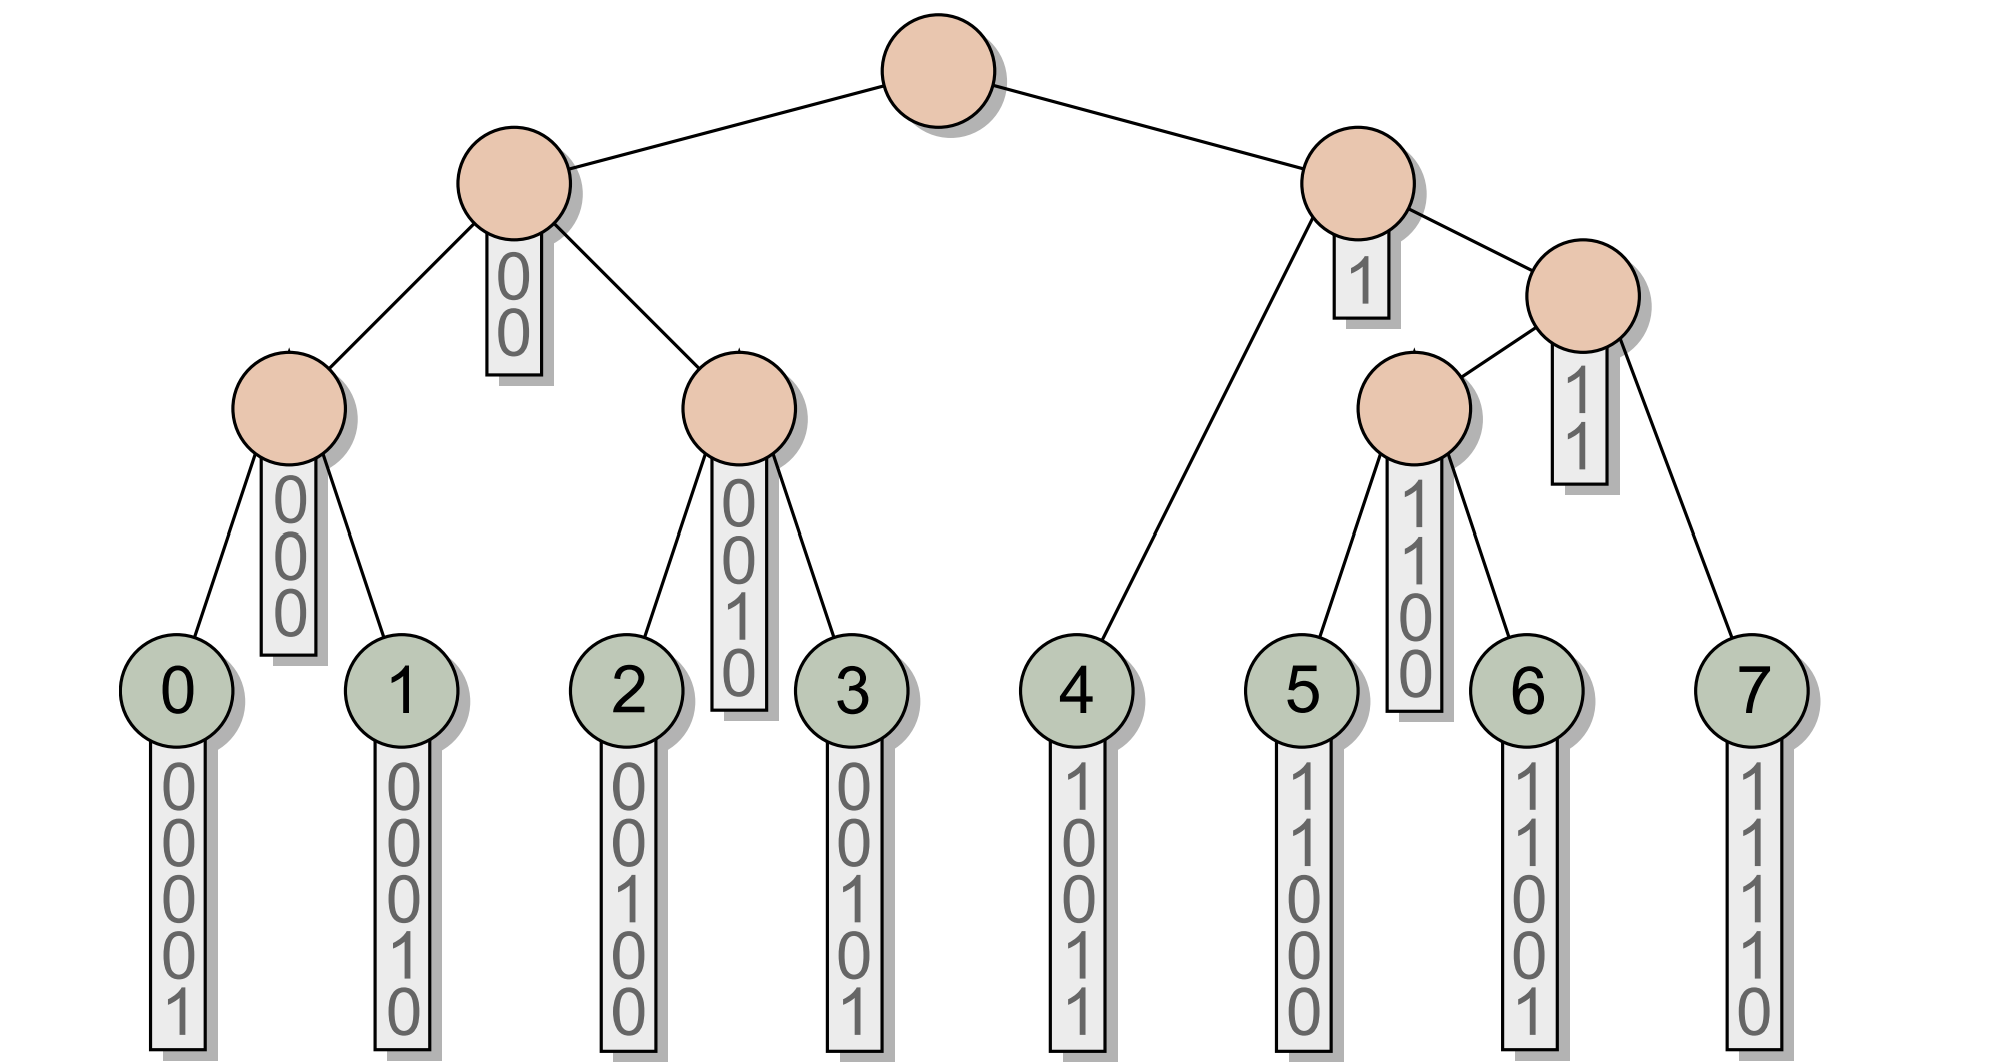
\includegraphics[height=5cm]{radix}
    \caption{Example radix tree. Image credit \cite{bvh_build}}
    \label{image radix tree}
\end{figure} 


In order to construct radix trees in parallel, the algorithm\cite{bvh_build} establishes a connection between node indices and keys through a specific tree layout, which enables interior nodes to be built simultaneously with their children. The layout stores interior and leaf nodes in two separate arrays, $I$ and $L$. The leaf array is sorted increasingly, and the interior array is arranged such that
\begin{enumerate}
    \item The root of the tree is at $I_0$.
    
    \item For each interior node $n$, which covers keys $k_i,...,k_j$, and splits at $k_\gamma$: the left child is stored at $I_\gamma$ if it is also an interior node, or at $L_\gamma$ if it is a leaf. Similarly, the right child is stored at either $I_{\gamma+1}$ if it is interior, or at $L_{\gamma+1}$ if it is a leaf.
\end{enumerate}

Notice that, these two rules enforces a special property: the index of an interior node coincides with the index of either its leftmost leaf descendent, or its rightmost leaf descendent. This property is visualized in the following image, where each vertical bar represents the range of keys covered by an interior node.
\begin{figure}[H]
    \centering
    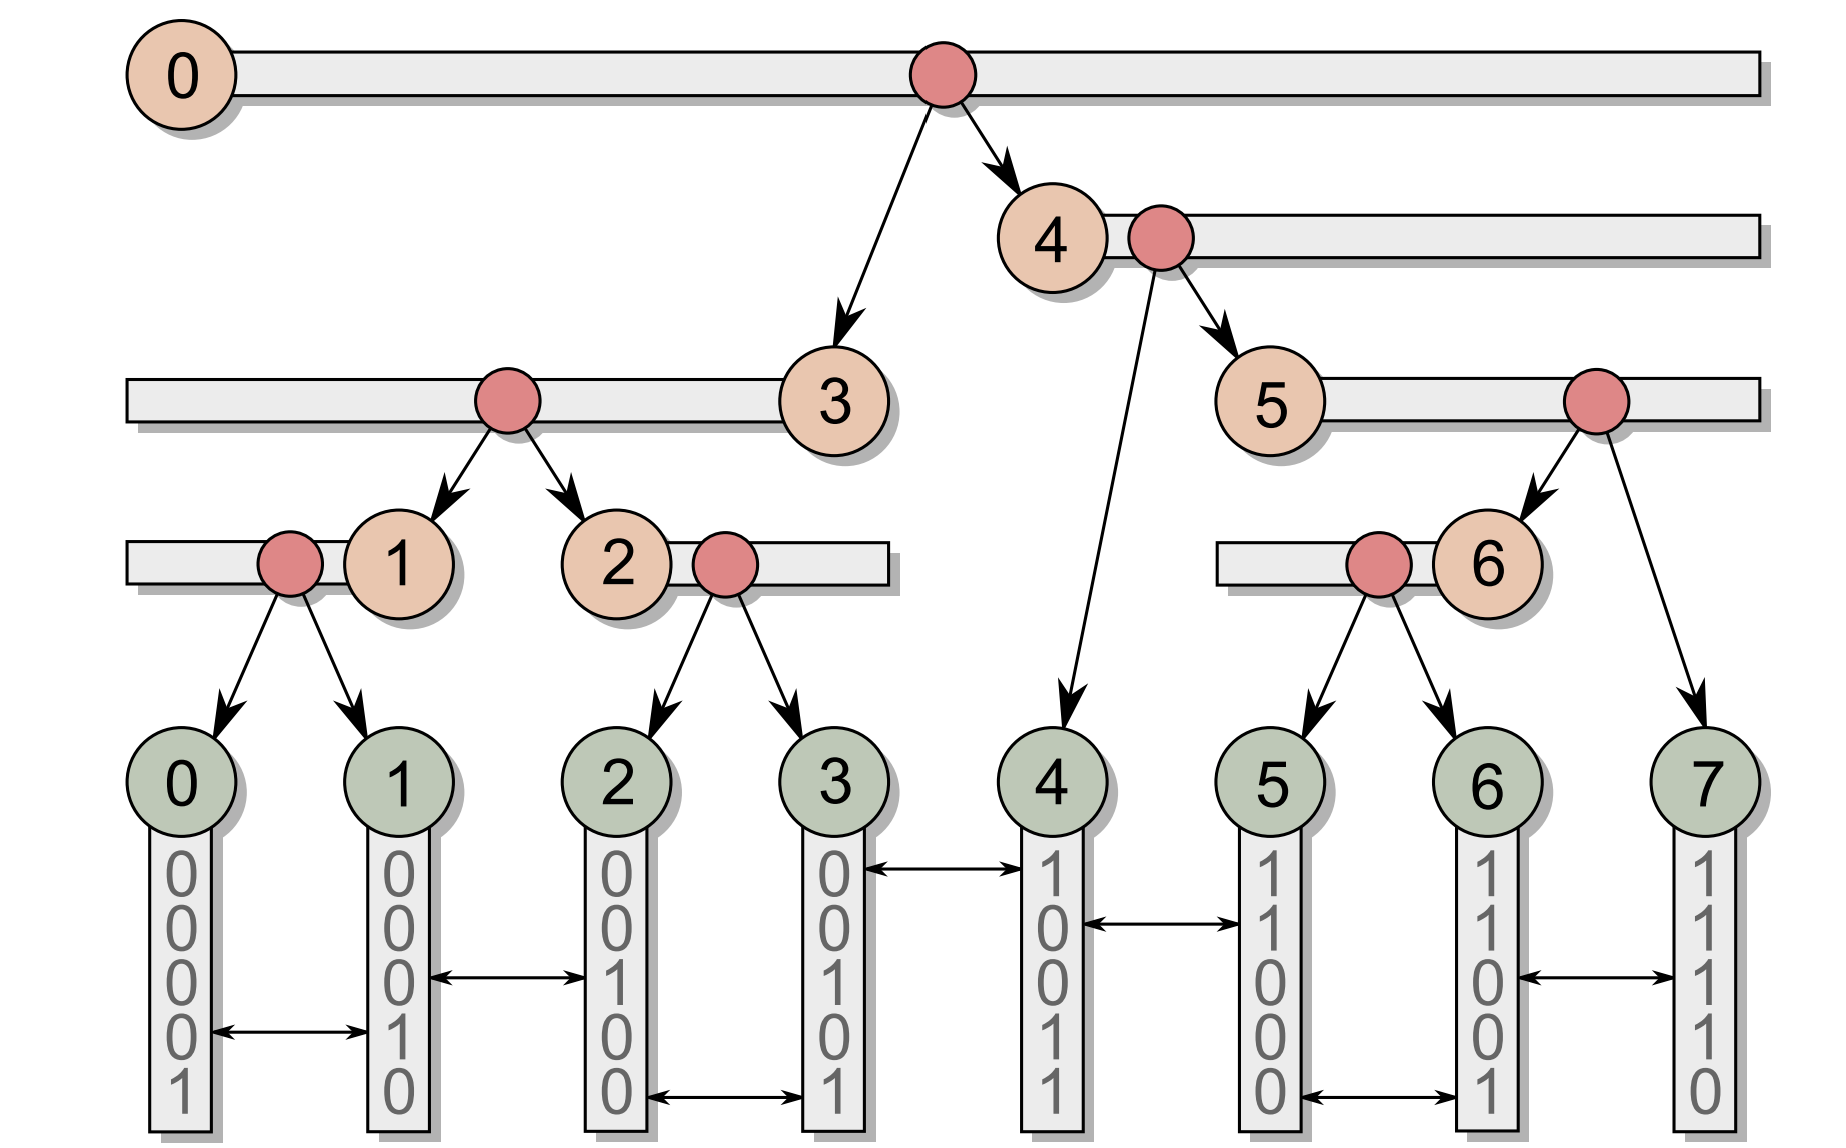
\includegraphics[height=5cm]{radix_layout.png}
    \caption{Radix tree storage layout. Image credit \cite{bvh_build}.}
\end{figure}

Given an interior node, it is not too hard to find out whether its index correspond to the leftmost descendent, or the rightmost one. More precisely, for the interior node $I_{x}$, it suffices to compare $\delta(x,x+1)$ and $\delta(x,x-1)$. If the former is larger, then $x$ must be the index of the leftmost descendent, and otherwise $x$ coincides with the rightmost descendent. Furthermore, the smaller value of $\delta(x,x+1)$ and $\delta(x,x-1)$ provides a minimum threshold of the maximum common prefix length $\delta(i,j)$ for $I_x$, that is, $\delta(i,j)> \text{min}(\delta(x,x+1),\delta(x,x-1))$. This is because, the minimum of $\delta(x,x+1)$ and $\delta(x,x-1)$ must equal the maximum common prefix length of the parent of $I_x$, and since $L_x$ is the children, it must have a greater maximum common prefix length. 

At this point, the algorithm knowns one of $i$ and $j$, and it also knows a lower-bound $\delta_{\text{min}}$ for $\delta(i,j)$. Without loss of generality, assume that the leftmost index $i$ is known. Notice that, $j$ is a value that satisfies $\delta(i,j)>\delta_{\text{min}}$, and it must be the maximum index that does so. Thus, it suffices to perform a binary search in the interval $[i+1,N]$, and find the largest $j$ that satisfies $\delta(i,j)>\delta_{\text{min}}$. 

Having computed the leftmost and rightmost descendants $i,j$ and the maximum common prefix length $\delta(i,j)$, it only remains to identify the index of the two children, $\gamma$ and $\gamma+1$. Notice that, since $\gamma$ is the rightmost index that still belongs in the left child, it is known that $\delta(i,\gamma)>\delta(i,j)$, and $\gamma$ is the largest index in $[i,j]$ that satisfies this property. Thus, it is again straightforward to use binary search to find $\gamma$. 

For each internal node $I_x$, the algorithm identifies its two children without requiring the children to have been constructed already. Thus, the algorithm can be parallelized across all nodes. The following pseudo-code summarizes this procedure:

\begin{algorithm}[H]
    \label{algo construct radix tree}
    \SetKwProg{Fn}{Function}{:}{end}
    \ForEach{\upshape internal node $L_x$ \textbf{in parallel}}{
        $\delta_{\text{min}} := \text{min}(\delta(x,x+1),\delta(x,x-1))$ \;
        \uIf{$\delta(x,x+1)>\delta(x,x-1)$}{
            $i:=x$\;
            Binary search to find the largest $j$ such that $\delta(i,j)>\delta_{\text{min}}$\;
        }
        \Else{
            $j:=x$ \;
            Binary search to find the smallest $i$ such that $\delta(i,j)>\delta_{\text{min}}$\;
        }
        Binary search to find the biggest $\gamma$ such that $\delta(i,\gamma)>\delta(i,j)$\;
        Left child is $I_{\gamma}$ as long as $i\neq \gamma$, and $L_{\gamma}$ otherwise\;
        Right child is $I_{\gamma+1}$ as long as $j\neq \gamma+1$, and $L_{\gamma+1}$ otherwise\;
        

    }
    \caption{Parallel Binary Radix Tree Construction}
\end{algorithm} 

~ 

One caveat with this algorithm is that no duplicates are allowed in the keys $k_0,...,k_{N-1}$. However, morton codes for two geometries could potentially be identical, if they're really close together. This problem can be easily taken care of by appending extra bits after the morton code and ensuring that all binary keys are distinct.

Having constructed the binary radix tree, it only remains to convert it into a BVH by computing an AABB for each node. This can be done in parallel by having all threads start at leaf nodes, move up the tree, and repeatedly compute the AABB for the current node along the way. Whenever two sibling threads move up to process a common parent, the two threads carry out a simple consensus operation to decide which thread should drop out and terminate. 

%\enlargethispage{3\baselineskip}

This project implemented this BVH construction on GPUs using CUDA. Thanks to the massively parallel nature of this algorithm, the project observed that the running time of this BVH construction algorithm is almost negligible ($\sim$50ms for 1 million primitives) compare to the cost of the actual path-tracing phase.


\subsection{BVH Optimization}
The BVH trees constructed by the algorithm from the previous section can immensely accelerate intersection detections and thus rendering. However, the quality of these trees are still quite poor compared to trees that are generated with the guidance of the SAH heuristic. To address this issue, this project implements the algorithm described int \cite{bvh_optimize}, which optimize existing BVH trees. With little running time cost, this optimization step boosts the rendering efficiency by about $300\%$.

It is believed that finding the optimal tree under the SAH heuristic is NP-hard\cite{bvh_optimize}, however, the algorithm follows the intuition that if the tree is optimal in every local \textit{treelet}, the entire tree would be somewhat optimal. Formally, a \textit{treelet} of size $n$ rooted at some node is defined to be a collection of immediate descendants of the root, consisting of $n-1$ internal nodes and $n$ leaf nodes (which can still be internal nodes in the complete tree). The algorithm solves the SAH optimization problem using dynamic programming for each treelet of size 7, in hopes that these local transformations improve the structure of the entire tree. 

\begin{figure}[H]
    \centering
    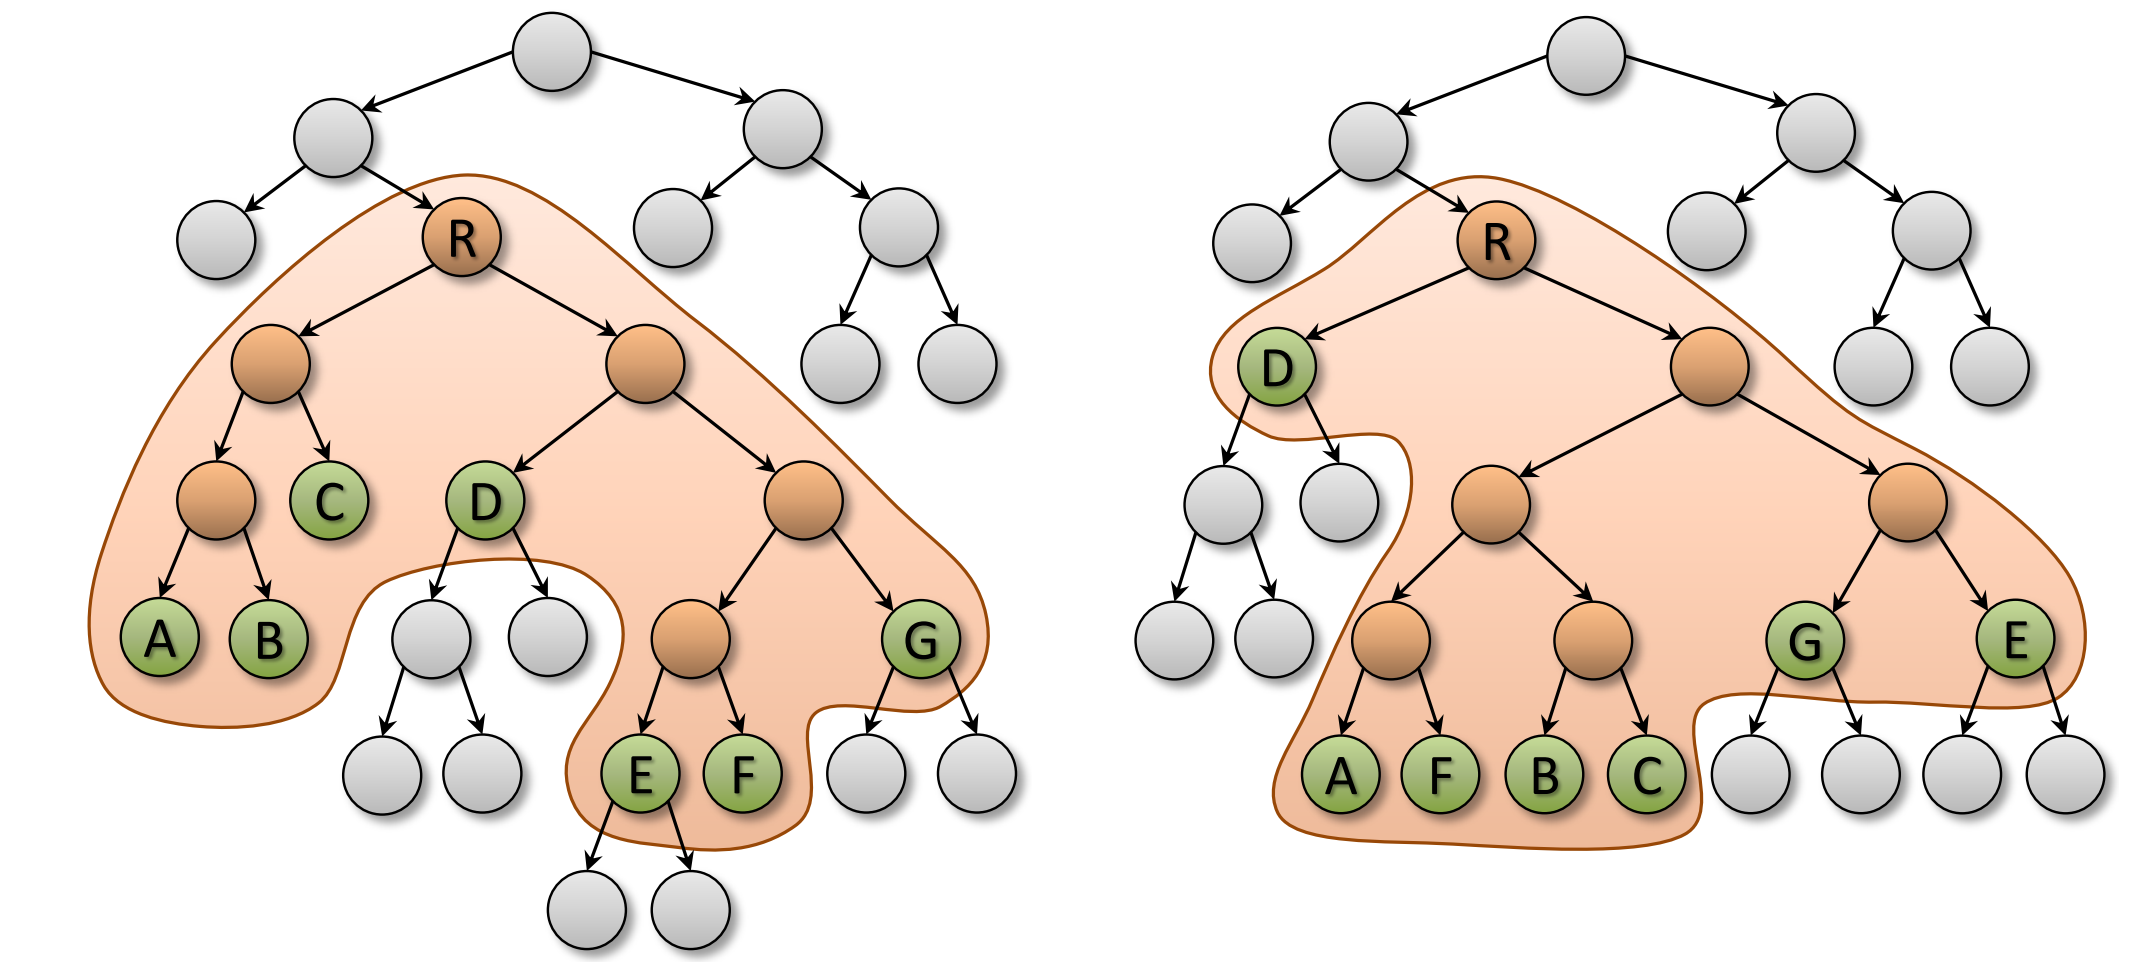
\includegraphics[height=5cm]{treelet.png}
    \caption{A treelet of size 7 and how it can be transformed. Image credit \cite{bvh_optimize}}
\end{figure}
For each internal node $n$, the algorithm defines its cost to be 
\begin{align*}
    C(n) = 
    \begin{cases}
        C_i A(n) + C(n_l) + C(n_r) &\text{if $n$ is an interior node in the full BVH}\\
        C_l A(n) &\text{if $n$ is a leaf node in the full BVH}\\
    \end{cases}
\end{align*}
where $n_l$ and $n_r$ are the left and right child. The cost defined this way is exactly the SAH cost multiplied by a constant factor of $A(root)$. For each internal node $n$ that is the root of a treelet of size 7, the algorithm optimizes $C(n)$ by finding the optimal structure of a local treelet. If more than one treelet of size 7 is rooted at $n$, the algorithm operates on the one where the leaves have the greatest surface area, which maximizes the potential for improvements. 

The algorithm optimizes treelets using dynamic programing. Specifically, it optimizes subsets of the leaves of increasing size, and memoize intermediate results. When working a subset of size $n$, it suffices to enumerate all possible binary partitions of this subset, and use memoized results to obtain optimal tree structure for each partition. Then, when the entire set of leaves is optimized, the treelet itself is also optimized. The procedure for optimizing each treelet is given in the following pseudo-code:

\begin{algorithm}[H]
    \label{algo optimize treelet}
    \SetKwProg{Fn}{Function}{:}{end}
    Create memoization array $C_{opt}$ of size $2^7$, indexed by subsets of the leaves (empirically represented as bitmaps by a 7-bit integers)\;
    \ForEach{leaf node $n$ of the treelet}{
        $C_{opt}[\{n\}] := C(n)$\;
    }
    \For{$k$ from $2$ to $7$}{
        \ForEach{subset $S$ of the leaves of size $k$}{
            $C_{opt}[S] := \infty$\;
            $A(S) :=$ surface area of the AABB that encloses all primitives in $S$\;
            \ForEach{pair of disjoint nonempty subsets $U,V$, where $U\cup V=S$}{
                $thisCost := A(S)C_i + C_{opt}[U] + C_{opt}[V]$\;
                \If{$thisCost<C_{opt}[S]$}{
                    $C_{opt}[S] := thisCost$\;
                    Record $(U,V)$ as current best partition for $S$\; 
                }
            }
        }
    }
    Restructure the treelet using the best partitions found\;
    \caption{Treelet Optimization}
\end{algorithm} 

~

For treelets rooted at the same level in the BVH, this optimization step can be parallelized because the treelets do not overlap. Thus, this project implemented the algorithm in GPU, where nodes across each level are processed in parallel. Again, this step is extremely efficient, taking around 200ms for a scene with 1 million triangle. This cost is extremely low compared to the actual rendering time.

\thispagestyle{empty}
\enlargethispage{5\baselineskip}

Interestingly, this optimization step does not reach a fixed point after optimizing each treelet once. The following image plots how the SAH cost (and thus rendering cost) changes when the BVH for a scene is optimized repeatedly. This project runs the optimization for 3 rounds for each scene, which almost always reduces SAH cost to one third of the origin value.

\begin{figure}[H]
    \centering
    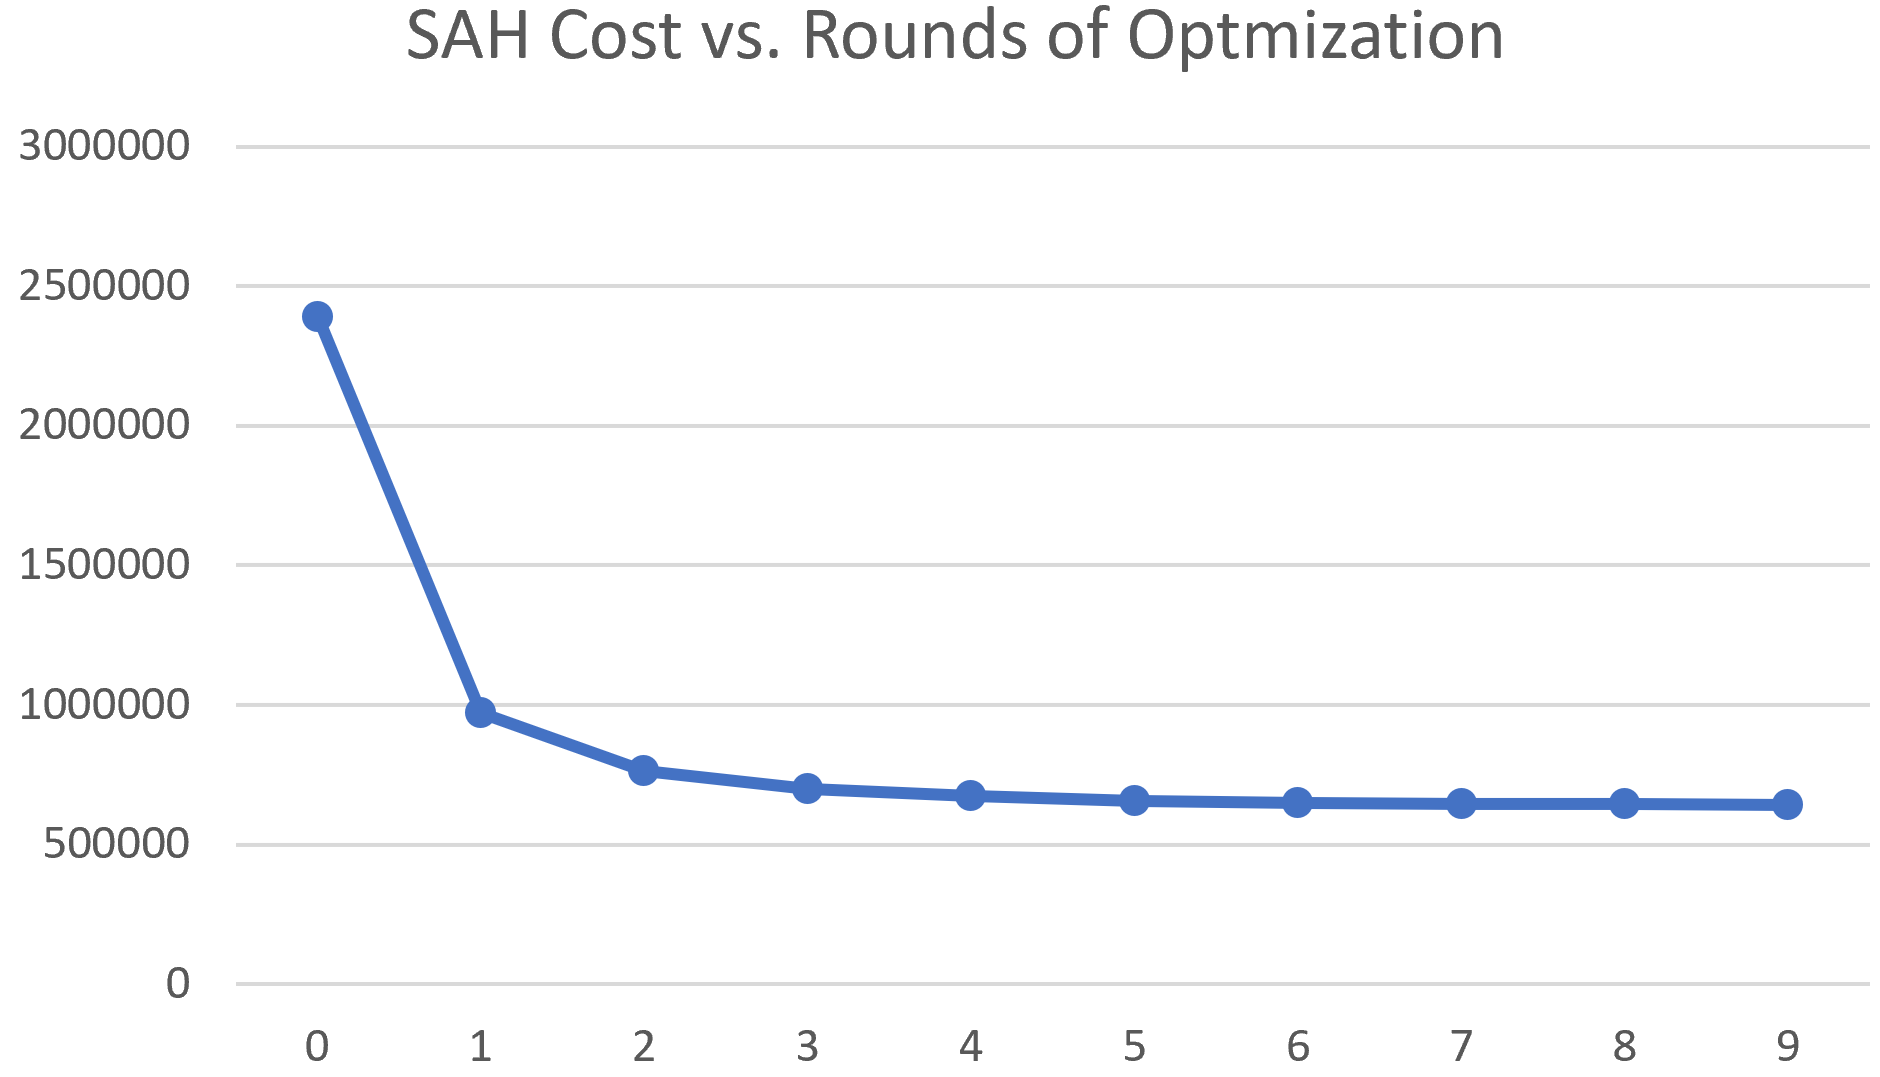
\includegraphics[height=5cm]{opt_rounds}
\end{figure}



%next line adds the Bibliography to the contents page
\addcontentsline{toc}{chapter}{Bibliography}
%uncomment next line to change bibliography name to references
%\renewcommand{\bibname}{References}
\bibliography{refs}        %use a bibtex bibliography file refs.bib
\bibliographystyle{plain}  %use the plain bibliography style

\end{document}

